%%%%%%%%%%%%%%%%%%%%%%%%%%%%%%%%%%%%%%%%%%%%%%%%%%%%%%%%%%%%%%%%%%%%%%
%%%%%%%%%%%%%%%%%%%%%%%%%%%%%%%%%%%%%%%%%%%%%%%%%%%%%%%%%%%%%%%%%%%%%%%
%%%%%%%%%%%%%%%%%%%%%%%%%%%%%%%%%%%%%%%%%%%%%%%%%%%%%%%%%%%%%%%%%%%%%%%
%%%%%%%%%%%%%%%%%%%%%%%%%%%%%%%%%%%%%%%%%%%%%%%%%%%%%%%%%%%%%%%%%%%%%%%
\chapter{\emph{ProbOnto} -- Ontology/Knowledge Base of Probability Distributions}
\label{ch:ProbOnto}


\paragraph{Background}
When encoding probabilistic uncertainties using a parametric distribution its name and 
parameters are sufficient to specify it in an unambiguous way as 
in most cases such parameter set is unique. But, because for a number of cases 
two or more parameterisations exist, one needs to be precise what 
parameters are used when referring to a distribution, otherwise one might 
end up with a wrong model (see for an example Figure \ref{fig:whatCanGoWrong}).
For this purpose an external standard reference is very useful as it allows to 
considerably reduce the effort of declaring the required distribution in a language 
such as MDL or PharmML.

\begin{figure}[htb!]
\centering
\begin{tabular}{cc}
 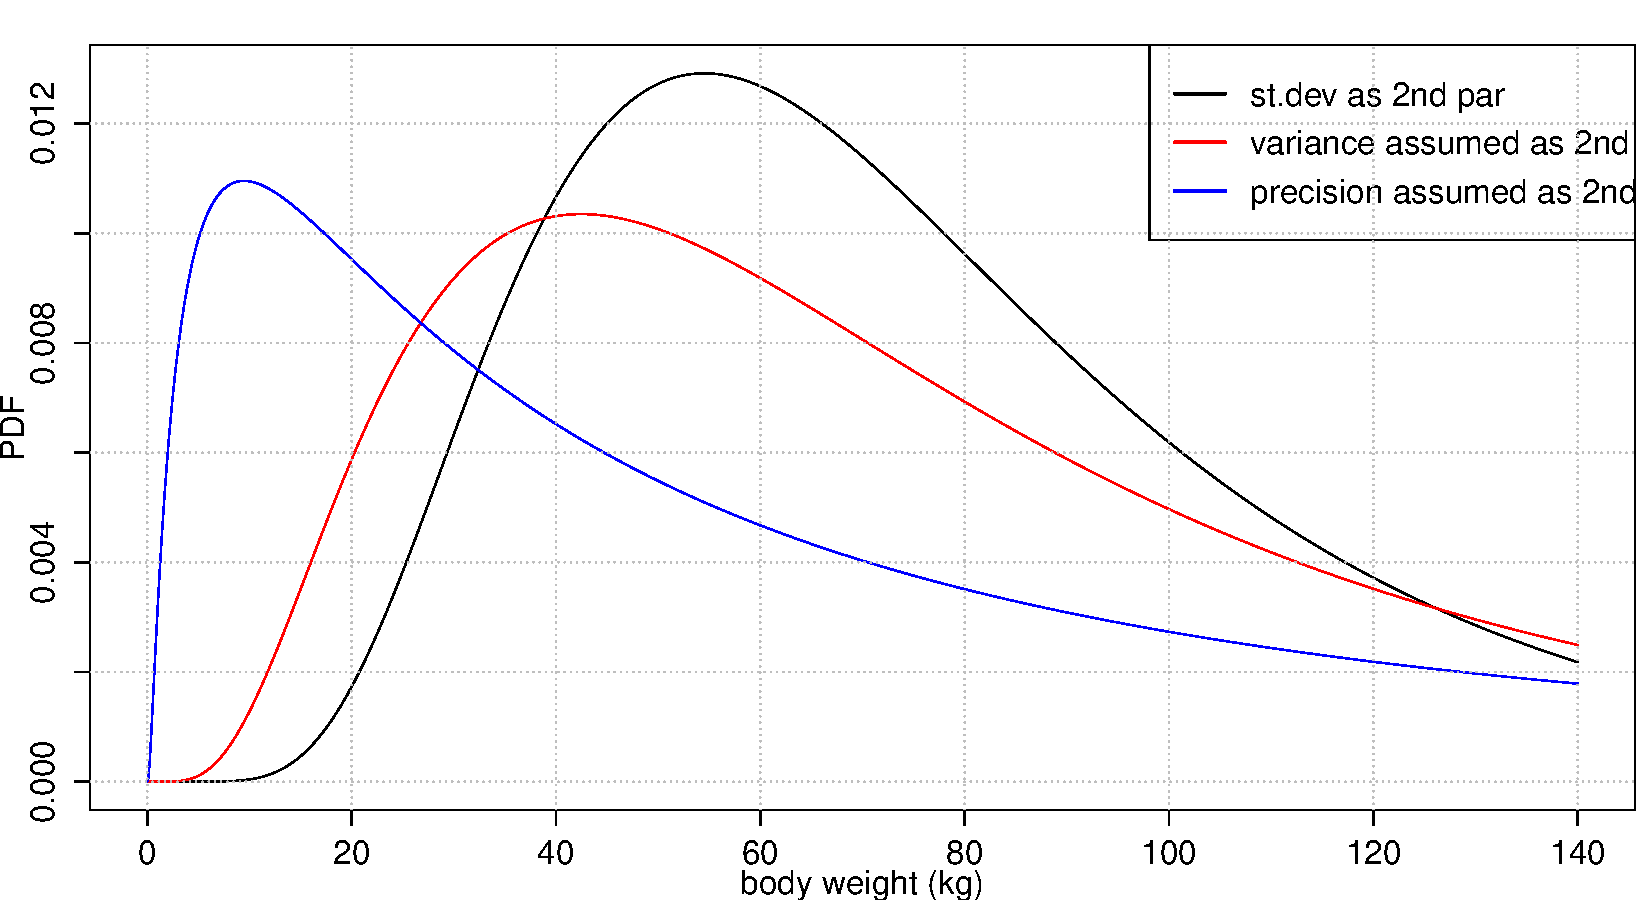
\includegraphics[width=140mm]{pics/whatCanGoWrong}
\end{tabular}
\caption{Illustration of possible model misspecification when using incorrect 
parameterisation. (1) The black curve corresponds to a log-normal 
distribution of body weight, $\mathcal {LN}(\mu\!=\!\log(70),\sigma\!=\!0.5)$, the 
intended parameterisation. (2) Here it was mistakenly assumed that 0.5 corresponds 
to the variance and calculation of standard deviation as required by the R function 
\emph{dlnorm} gives $\sigma = \sqrt{0.5}=0.707$ (red). (3) Here the modeller 
assumed that the 2nd input value corresponds to the precision and calculated the 
standard deviation as $\sigma = 1/\sqrt{0.5}=1.41$ (blue). Small numerical 
differences in $\sigma$, on the log-scale, result in significant differences on the natural scale.}
\label{fig:whatCanGoWrong}
\end{figure}

Until now, we have been relying on the UncertML, \cite{uncertml3:2014}, 
which provides means to encode in MDL/PharmML a range of continuous and 
discrete uni/multi-variate probability distributions. However, from the perspective 
of PharmML, it has several limitations as described in section \ref{sec:uncertmlLimits}. 

\paragraph{Idea} The initial motivation for \emph{ProbOnto} was to create an ontology of probability 
distributions purely for annotation purposes. Many resources are available online 
and in printed format but no proper ontology exists so far\footnote{For 
example, the Statistics Ontology, STATO, \url{http://stato-ontology.org/}, provides 
for most distributions merely a link to an external reference/definition. No parameters
or related functions and quantities are defined in the ontology making their annotation
impossible. Other ontologies, we have analysed number of them featured in the 
BioPortal, \cite{noy2009bioportal}, suffer from equivalent limitations
as they are designed in a similar way.}.  
Similarly, the databases of distributions available online come with analog issues. 
The largest and most comprehensive known to us collection of probability distributions, the 
UUPDE, \cite{UUPDE:2013}, with up to 60 properties for each of its 
500 probability distributions is an invaluable resource for parametric distributions. 
Unfortunately, it comes with univariate cases only and lacks number of relevant for us 
distributions, doesn't provide references or parameter names making its use in our 
context impracticable\footnote{Another case is Distributome, 
\url{http://www.distributome.org/}, comes with an impressive and well referenced collection
of 90+ distributions but doesn't contain many of relevant for us types and/or 
parameterisations and is limited to univariate parametric ones.}. \\
It turns out that \emph{ProbOnto} can be very helpful in designing a flexible 
alternative for UncertML with many additional features.
It can be used e.g. in PharmML or other target tools/languages \emph{both} 
as ontological resource for annotation purposes and as a knowledge base, 
see next section for their definitions, to provide the means to specify a wide range 
of distributions and distribution related functions and quantities.

In fact, such solution is indispensable in the face of requirements 
posed by models we would like to encode currently and in the foreseeable future. 

%%%%%%%%%%%%%%%%%%%%%%%%%%%%%%%%%%%%%%%%%%%%%%%%%%%%%%%%%%%%%%%%%%%%%%
\section{Ontology versus Knowledge Base}
\begin{description}
\item[Ontology] is a formal representation of a domain of knowledge. It is an abstract entity 
defining the vocabulary for a domain and the relations between concepts.
However, an ontology doesn't specify how that knowledge is stored 
(as physical file, in a database, or in some other form), and how the knowledge 
can be accessed.
\item[Knowledge base] is a physical artifact. It is a database, a repository of information 
that can be accessed and manipulated in some predefined fashion.
\end{description}
The knowledge in a knowledge base is modelled according to rules and relationships 
defined in an ontology.

%%%%%%%%%%%%%%%%%%%%%%%%%%%%%%%%%%%%%%%%%%%%%%%%%%%%%%%%%%%%%%%%%%%%%%
\section{Limitations of the application of UncertML in PharmML}
\label{sec:uncertmlLimits}
Although very useful to a certain extent, there are limitations in
the design and scope of UncertML making the encoding of some 
probability distributions cumbersome or even impossible, see examples below. 
Here some known limitations (in the order of severity):
\begin{itemize}
\item
it doesn't support the assignment of expressions for distribution parameters or 
the specification of block references, which is required if the parameter in question 
is defined elsewhere in the model. 
\item
it doesn't cover many distributions used in Pharmacometrics, e.g. 
\begin{itemize}
\item 
multivariate continues distributions such as Inverse-Wishart
\item
discrete distributions such as Generalized Poisson, Zero-inflated Poisson etc.
\item
or alternative parameterisations for distributions such as Negative Binomial, 
Log-Normal etc.
\end{itemize}
\item
\xelem{degreesOfFreedom} parameter element of the Wishart distribution doesn't support
referencing a variable (required for Bayesian inference) -- a known bug/limitation 
but with no solution for now.
\item
UncertML is a reference resource for distributions but does not provide 
mechanisms to retrieve programmatically related functions and
quantities.  
\item
Negative Binomial comes with different formulation and interpretation 
(as opposed to just different parameterisation). UncertML features an option which is 
rarely seen in the literature (and different compared to R, Matlab and winBUGS) 
which might remain unnoticed to the unexperienced user leading to false results.
A detailed discussion can be found in the appendix \ref{app:sec:NB1discussion}.
\end{itemize}
Other minor issues:
\begin{itemize}
%\item
%changes/updates in the unpublished version 3.0 happen without providing 
%documentation change-log.
\item
the implementation of \xelem{MultivariateNormalDistribution} requires the specification 
of the \xatt{dimension} attribute of the covariance matrix -- although this can be estimated
it requires unnecessary calculations when translating models to PharmML. 
\item
every extension requires changes in the already complex XML schema.
\item
doesn't support the precision parameter, $\tau$, used in winBUGS  
rather then standard deviation or variance and precision matrix, $T$, instead 
of covariance matrix $\Sigma$, see tables \ref{figTable:univariates} and \ref{figTable:multivariates}.
\item
version 3.0 which we currently use is not yet released publicly, the UncertML website 
is not updated and 3.0 documentation is not available.
\end{itemize}

\paragraph{UncertML extension} A seemingly easy solution would be to extend UncertML 
but to do so, it would mean to introduce major extensions and changes to its 
current XML schema. Only the support of the most important missing features would 
de facto require to rewrite the entire standard, as UncertML doesn't possess the 
structure to encode even basic algebraic expressions. And because it would most 
certainly result in a different, compared to PharmML, mathematical notation we would 
be faced with inconsistent, layered and/or overlapping schemas difficult to handle and 
to process.

\paragraph{Suggested way forward} ProbOnto offers an alternative solution allowing
to avoid all the limitations listed above while providing number of additional features
and means to build in a very flexible probability distribution support in MDL, PharmML 
and other languages/tools within DDMoRe and beyond. 

%%%%%%%%%%%%%%%%%%%%%%%%%%%%%%%%%%%%%%%%%%%%%%%%%%%%%%%%%%%%%%%%%%%%%%
\section{ProbOnto Features}
\begin{itemize}
\item
General 
\begin{itemize}
\item
Covers more then 70 distributions and alternative parameterisations (as of 3$^{rd}$ Sept 2015).
\item
Supports encoding of univariate mixture distributions and truncation bounds (open/closed).
\item
Allows for easy encoding of distributions and related functions in target 
tools/languages thanks to its generic format.
\item
Doesn't enforce specific implementation in target tools.
\item
In PharmML only few extensions were required to provide flexible encoding support
for all distributions and their features, see section \ref{sec:workingProbOnto}.
\item
Collection of supported distributions, see appendix \ref{ch:probontoAppendix} for 
some selected types and their essential features, is easily extendable 
without non or limited impact on the PharmML structure.
\item
All mathematical functions and quantities are available in Latex and  for a number 
of functions R-code is provided.
\end{itemize}
\item
ProbOnto as Ontology
\begin{itemize}
\item
It can be used to annotate statistical models based on supported probability 
distributions, e.g. their name, parameters, truncation bounds, their defining 
functions and quantities.
\end{itemize}
\item
ProbOnto as Knowledge Base
\begin{itemize}
\item
Provides for each distribution either PDF or PMF and in many cases also 
other distribution related functions such as CDF, hazard and survival functions 
-- the level of coverage depends on the particular distribution. 
%see Appendix \ref{ch:probontoAppendix}.
\item
Provides related quantities such as mean, median, mode, variance etc.
\item
Provides other info about \emph{support/range} and relationships to other distributions.
\end{itemize}
\end{itemize}
The distribution collection and their features are based on
probability distribution pages of the english Wikipedia\footnote{See the list of 
distributions on Wikipedia at \url{https://en.wikipedia.org/wiki/List_of_probability_distributions}}, 
Forbes et al. 2011 \cite{forbes2011statistical}, Leemis et al. 2008 \cite{Leemis:2008tg}, 
Song \& Chen 2011 \cite{song2011eighty}, and 
Wolfram MathWorld \cite{weisstein2007wolfram}.

%%%%%%%%%%%%%%%%%%%%%%%%%%%%%%%%%%%%%%%%%%%%%%%%%%%%%%%%%%%%%%%%%%%%%%
\subsection{Features under construction}
The following features are under construction and not available in the current 
release
\begin{itemize}
\item
truncation bounds -- supported already for all univariate distributions but an extension 
to multivariate distributions is needed.
%\item
%mixture models - added but more testing required -- see example 'Poisson with mixture distribution', PMIX.
\item
non-parametric distributions.
\end{itemize}
They are available to certain extend in UncertML, which can be used instead for the time being, if required.


%%%%%%%%%%%%%%%%%%%%%%%%%%%%%%%%%%%%%%%%%%%%%%%%%%%%%%%%%%%%%%%%%%%%%%%
\section{Working with ProbOnto}
\label{sec:workingProbOnto}
The subsequent chapters come with a number of examples of ProbOnto use
but it is worth to point out two basic implementation rules 
\begin{itemize}
\item 
The name of a distribution, encoded in the \xelem{ProbOnto name="..."} tag, 
where instead of the dots one of the 'Code names' assigned to each distribution in ProbOnto
must be used. 
\item
The same holds for the parameters of a distribution, encoded in the \xelem{Parameter name="..."} tag. 
Note that the order of parameters doesn't matter. 
\end{itemize}
%We have found in the literature many instances of different names being used 
%for parameters a given distributions. 
To remain consistent with the nomenclature used so far in PharmML and MDL (which
was based on UncertML vocabulary) the majority of parameter's \emph{code names} is 
identical to those used in UncertML. For new distributions and their parameters we have 
defined the most common names used in the literature. 
The  \emph{code names} are collected in the tables \ref{figTable:univariatesCodes}, 
\ref{figTable:multivariatesCodes} and \ref{figTable:mixtures}. 

\begin{example}
The implementation of the negative binomial model illustrates how this works. There are many 
parameterisations for this distribution but the version with Poisson intensity, $\lambda$, 
and over-dispersion, $\tau$, as parameters, with the code name, \emph{NegativeBinomial2}, 
is frequently used in discrete data models.
\lstset{language=XML}
\begin{lstlisting}
    <Distribution>
        <ProbOnto name="NegativeBinomial1">
            <Parameter name="rate">
                <ct:Assign>
                    <ct:SymbRef blkIdRef="pm1" symbIdRef="rabbit"/>
                </ct:Assign>
            </Parameter>
            <Parameter name="overdispersion">
                <ct:Assign>
                    <ct:SymbRef blkIdRef="pm2" symbIdRef="piggy"/>
                </ct:Assign>
            </Parameter>
        </ProbOnto>
    </Distribution>
\end{lstlisting}
%	
According to the rules, the names of the distributions and their parameters 
must be the code names defined by ProbOnto, see table \ref{figTable:multivariatesCodes}. 
The user can then assign any symbols to the parameters,
with \emph{rabbit} for \emph{rate}, defined in 
parameter model \xatt{pm1} and \emph{piggy} for \emph{overdispersion}, 
defined in parameter model \xatt{pm2}.
%effort required in PharmML and other target 
%tools to make use of ProbOnto is reduced to minimum.
\end{example}

\subsection{New elements supporting ProbOnto}
The following elements are new in this version to support ProbOnto encoding 
\begin{itemize}
\item
\xelem{ProbOnto} tag with the \xatt{name} attribute for the distribution code names
 with children elements
\begin{itemize}
\item
\xelem{Parameter} with the \xatt{name} attribute for the parameter code names. 
It can be assigned any expression.
\item
\xelem{LowerTruncationBound} and \xelem{LowerTruncationBound} to indicate the
truncation bounds for univariate distributions with attribute \xatt{type} which can
be either \emph{closed} or \emph{open}.
\item
\xelem{MixtureComponent} with the \xatt{name} attribute for the code name of mixture 
component.
\end{itemize}
\end{itemize}



\section{Annotation of models with ProbOnto ontology}

\subsection{Implementation in PharmML}

The following code shows the typical Poisson model implementation
\lstset{language=XML}
\begin{lstlisting}
            <PMF linkFunction="log">
                <Distribution>
                    <ProbOnto id="X1" name="Poisson">
                        <Parameter id="X2" name="rate">
                            <ct:Assign>
                                <ct:SymbRef blkIdRef="pm1" symbIdRef="lambda"/>
                            </ct:Assign>
                        </Parameter>
                    </ProbOnto>
                </Distribution>
            </PMF>
\end{lstlisting}

\subsection{Annotation of PharmML}

Notice that in the above sniper of code the elements defining the distribution used, \xelem{ProbOnto},  
and its parameter, \xelem{Parameter} are given identifiers, \xatt{id="X1"} and \xatt{id="X2"}, respectively.
This allows us to annotate these elements so that we can make explicit their intended interpretation. Using the PharmML metadata annotation schema, we would record such interpretation using the property {\emph{has-interpreted-type}. In what follows, 'ps' abbreviates the namespace for this schema and 'probonto' abbreviates the namespace for the ProbOnto ontology, part of the stack of ontologies used in PharmML annotation. 

\begin{quote}
\# The distribution element is interpreted as an instantiation of the Poisson distribution.

\emph{X1 ps:has-interpreted-type probonto:0000111.}

\# The parameter element is interpreted as an instantiation of the parameter element, $\lambda$, of the Poisson distribution.

\emph{X2 ps:has-interpreted-type probonto:0000114.}
\end{quote}

In ProbOnto, \emph{0000111} and \emph{0000114} are the identifiers for the Poisson distribution 
and its (unique) parameter, respectively. The two statements above encode the interpretation 
of the PharmML code defining the distribution. Such statements can in principle be generated automatically 
after processing the PharmML code.

Annotating the actual PharmML model and the element to which the distribution applies would involve 
more or a variation upon the above to the effect that the ProbOnto distribution is identified.

\subsection{Background Information is Contained in ProbOnto}

Given the annotation of the PharmML code linking to ProbOnto, we can then use ProbOnto to make explicit all the information that is packed into these two very terse annotation statements.

\subsubsection*{Underlying accessible knowledge about Poisson distribution}

We thus have access to the following regarding the distribution contained in the PharmML code (as much as is contained in the ProbOnto definition of the Poisson distribution):

\bigskip
\begin{tabular}{p{2cm}cl}
\textbf{name} & & Poisson (ID: 0000111)\\

\textbf{type} & & discrete \\

\textbf{variate} & & $k$, scalar \\

\textbf{support} & & $k \in \{0,1,2,3,\dots\}$
\end{tabular}
\bigskip \\
Additionally, we can obtain from ProbOnto the following type of information. 
\subsubsection*{Underlying accessible knowledge about the related functions}
%\subsubsection*{Functions}
\smallskip \noindent \hspace{.2cm} \textbf{PMF}
\begin{equation*}\frac{\lambda^k}{k!}e^{-\lambda}\end{equation*}
\smallskip \noindent \hspace{.2cm} \textbf{PMF in R}
\begin{verbatim}lambda^k/factorial(k) * exp(-lambda)\end{verbatim}
\smallskip \noindent \hspace{.2cm} \textbf{CDF}
\begin{equation*}\frac{\Gamma(\lfloor k+1 \rfloor,\lambda)}{\lfloor k \rfloor!}\end{equation*}
\smallskip \noindent \hspace{.2cm} \textbf{CDF in R}
\begin{verbatim}Igamma(floor(k+1), lambda, lower=F) / factorial(floor(k))\end{verbatim}
using \emph{Igamma} from \url{http://cran.r-project.org/web/packages/zipfR/zipfR.pdf}.

\subsubsection*{Underlying accessible knowledge about the (rate) parameter}

\noindent\begin{tabular}{p{2cm}cl}
\textbf{name} & & Poisson intensity  (ID: 0000114) \\
\textbf{type} & & scalar \\
\textbf{symbol} & & $\lambda$  \\
\textbf{definition} & & $\lambda \in R, \lambda > 0$
\end{tabular}
\bigskip 

The amount of information that may be encoded in ProbOnto is extensible. 
Thus,  via a very simple and direct mechanism of annotation that amounts to 
linking a distribution and its parameter(s) in a piece of PharmML code, we can
 inherit and obtain all the background relevant information. 
 This knowledge can be used either for our understanding and the validation of 
 our PharmML encoding or, with adequate software support, for processing by 
 tools. 
 
Currently, such extensive software support is not available but is part of the 
development path for PharmML and its implementation of ProbOnto. 

\begin{figure}[htb!]
\centering
  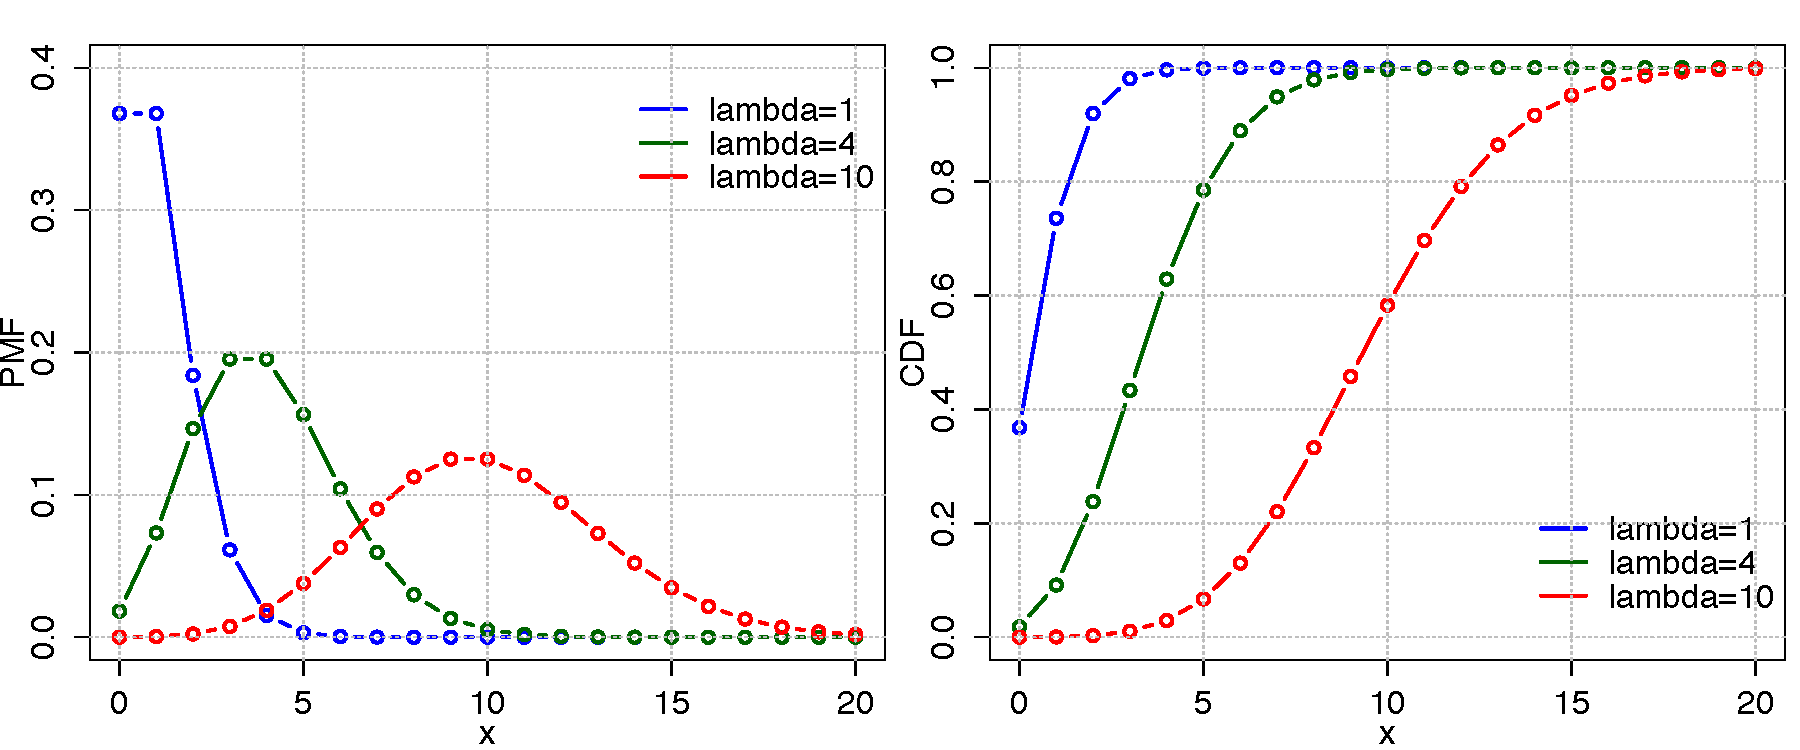
\includegraphics[width=140mm]{pics/Poisson.pdf}
 \caption{PMF and CDF of the Poisson distribution plotted using the R-code
 stored in ProbOnto.}
 \label{fig:PoissonExample}
\end{figure}


%%%%%%%%%%%%%%%%%%%%%%%%%%%%%%%%%%%%%%%%%%%%%%%%%%%%%%%%%%%%%%%%%%%%%%%
\section{Alternative parameterisations -- examples {\color{red} \scshape{updated}}}
\label{sec:altParams}
The existence of alternative parameterisations is apparent for number of reasons, 
such as model type, application area, available data and/or target tool -- e.g. BUGS using 
precision, $\tau$, rather then standard deviation or variance for a normal/log-normal
and a number of other distributions. Moreover, ProbOnto contains, wherever available, 
re-parameterisations formulas of distributions coming in different forms. 
This can be seen as an improvement of the inter-operability support between target 
tools supporting different parameter sets for a given probability density/mass function.

The needs for the support of re-parameterisation, e.g. between BUGS and R has been 
discussed before, \cite{lebauer2013translating}. The authors state that "[...] R and BUGS 
languages use different representations of common probability density 
functions, creating a potential for errors to occur in the implementation 
or interpretation of analyses that use both languages"). 

A few typical examples for alternative parameterisations are given in next sections.

\subsection{Negative binomial distribution} 
\label{subsec:altNB}
The available parameterisations are
\begin{itemize}
\item
Negative Binomial 1\,($r$, $p$) with r -- \emph{number of successes} and p -- \emph{success probability}
\begin{align}
P(k;r,p) = \binom {k+r-1}k p^r (1-p)^k, \quad k\in \{0,1,2,\dots \} \text{ number of failures} \nonumber
\end{align}

\item
Negative Binomial 4\,($r$, $p$) with r -- \emph{number of failures} and p -- \emph{success probability}
\begin{align}
P(k;r,p) = \binom {k+r-1}k (1-p)^r p^k, \quad k\in \{0,1,2,\dots \} \text{ number of successes} \nonumber
\end{align}

\item
Negative Binomial 2\,($\mu$, $\tau$), \cite{Plan:2009fk}, with $\mu$ -- \emph{mean} and $\tau$ -- \emph{over-dispersion},
\begin{align}
P(k;\mu,\tau) = \frac{\Gamma(k+\frac{1}{\tau})}{k!\; \Gamma(\frac{1}{\tau})} \Big(\frac{1}{1+\tau \mu} \Big)^{\frac{1}{\tau}} \Big(\frac{\mu}{\frac{1}{\tau} + \mu} \Big)^{k},\quad k\in \{0,1,2,\dots \}  \nonumber
\end{align}

\item
Negative Binomial 3\,($\mu$, $\phi$), \cite{stan-manual:2015}, %with $\lambda$ -- \emph{Poisson intensity} and $\tau$ -- \emph{over-dispersion},
\begin{align}
P(k;\mu,\phi) = \binom {k+\phi-1}k \Big(\frac{\phi}{\mu + \phi} \Big)^{\phi} \Big(\frac{\mu}{\mu + \phi} \Big)^{k},\quad k\in \{0,1,2,\dots \}  \nonumber
\end{align}
\end{itemize}
with NB2 being used in typical pharmacometric discrete data models, \cite{Plan:2009fk, Troconiz:2009fv}.
See appendix \ref{app:sec:NB1discussion} for a detailed discussion on the possible formulations. 
%The Wikipedia article\footnote{\url{en.wikipedia.org/wiki/Negative_binomial_distribution}, 
%section 'Alternative formulations'}, explains the reasons behind the various representations.

\subsubsection{Re-parameterisation formulas}
We give below the available re-parameterisations for the negative binomial
\begin{itemize}
\item 
\begin{description}
\item[NB1($r$, $p$) $\rightarrow$ NB2($\mu$, $\tau$)]:
$r \rightarrow \tau = 1/r; \quad p \rightarrow \mu = \frac{1-p}{p\tau}$

\item[NB2($\mu$, $\tau$) $\rightarrow$ NB1($r$, $p$)]:
$\tau \rightarrow r=1/\tau; \quad \mu \rightarrow p = \frac{1}{1+\tau \mu}$
\end{description}

\item 
\begin{description}
\item[NB1($r$, $p$) $\rightarrow$ NB3($\mu$, $\phi$)]:
$r \rightarrow \phi=r; \quad p \rightarrow \mu=\frac{r (1-p)}{p}$

\item[NB3($\mu$, $\phi$) $\rightarrow$ NB1($r$, $p$)]:
$\phi \rightarrow r=\phi; \quad \mu \rightarrow p=\frac{r}{\mu+r}$
\end{description}

\item 
\begin{description}
\item[NB2($\mu$, $\tau$) $\rightarrow$ NB3($\mu$, $\phi$)]:
$\mu \rightarrow \mu; \quad \tau \rightarrow \phi=1/\tau$

\item[NB3($\mu$, $\phi$) $\rightarrow$ NB2($\mu$, $\tau$)]:
$\mu \rightarrow \mu; \quad \phi \rightarrow \tau=1/\phi$
\end{description}

\item 
\begin{description}
\item[NB4($r$, $p$)] -- any re-parameterisations including this distribution 
would require reformulation of the support variable and the parameters,
see detailed explanation in the appendix \ref{app:sec:NB1discussion}. 
\end{description}

\end{itemize}



\subsection{Normal distribution}
Available parameterisations (see also Table \ref{figTable:logNormalParameterisations} 
with indication about their coverage in target tools) are
\begin{itemize}
\item
Normal1\,($\mu$, $\sigma$) with $\mu$ -- \emph{mean} and $\sigma$ -- \emph{standard deviation}, 
\begin{align*}
P(x;\boldsymbol\mu,\boldsymbol\sigma)= \frac{1}{\sigma \sqrt{2 \pi}}\exp\Big[-\frac{(x-\mu)^2}{2\sigma^2}\Big]
\end{align*}
\item
Normal2\,($\mu$, \emph{v}) with $\mu$ -- \emph{mean} and \emph{v} -- \emph{variance},
\begin{align*}
P(x;\boldsymbol\mu,\boldsymbol v)= \frac{1}{\sqrt{v} \sqrt{2 \pi}}\exp\Big[-\frac{(x-\mu)^2}{2v}\Big]
\end{align*}
\item
Normal3\,($\mu$, $\tau$) with $\mu$ -- \emph{mean} and $\tau$ -- \emph{precision} ($\tau=1/\sigma^2$)
\begin{align*}
P(x;\boldsymbol\mu,\boldsymbol\tau)= \sqrt{\frac{\tau}{2 \pi}} \Big[-\frac{\tau}{2}(x-\mu)^2\Big].
\end{align*}
\end{itemize}

\subsubsection{Re-parameterisation formulas}
In this case the recalculations between the representations are very simple
but are given here for the completeness
\begin{itemize}
\item 
\begin{description}
\item[N1($\mu$, $\sigma$) $\rightarrow$ N2($\mu$, $v$)]:
$\mu \rightarrow \mu; \quad \sigma \rightarrow v=\sigma^2$

\item[N2($\mu$, $v$) $\rightarrow$ N1($\mu$, $\sigma$)]:
$\mu \rightarrow \mu; \quad v \rightarrow \sigma = \sqrt{v}$
\end{description}

\item 
\begin{description}
\item[N1($\mu$, $\sigma$) $\rightarrow$ N3($\mu$, $\tau$)]:
$\mu \rightarrow \mu; \quad \sigma \rightarrow \tau=1/\sigma^2$

\item[N3($\mu$, $\tau$) $\rightarrow$ N1($\mu$, $\sigma$)]:
$\mu \rightarrow \mu; \quad \tau \rightarrow \sigma=1/\sqrt{\tau}$
\end{description}

\item 
\begin{description}
\item[N2($\mu$, $v$) $\rightarrow$ N3($\mu$, $\tau$)]:
$\mu \rightarrow \mu; \quad v \rightarrow \tau=1/v$

\item[N3($\mu$, $\tau$) $\rightarrow$ N2($\mu$, $v$)]:
$\mu \rightarrow \mu; \quad \tau \rightarrow v=1/\tau$.
\end{description}
\end{itemize}

\begin{figure}[htb!]
\centering
\begin{tabular}{cc}
% \includegraphics[width=140mm]{pics/CDF_17Dec} \\
 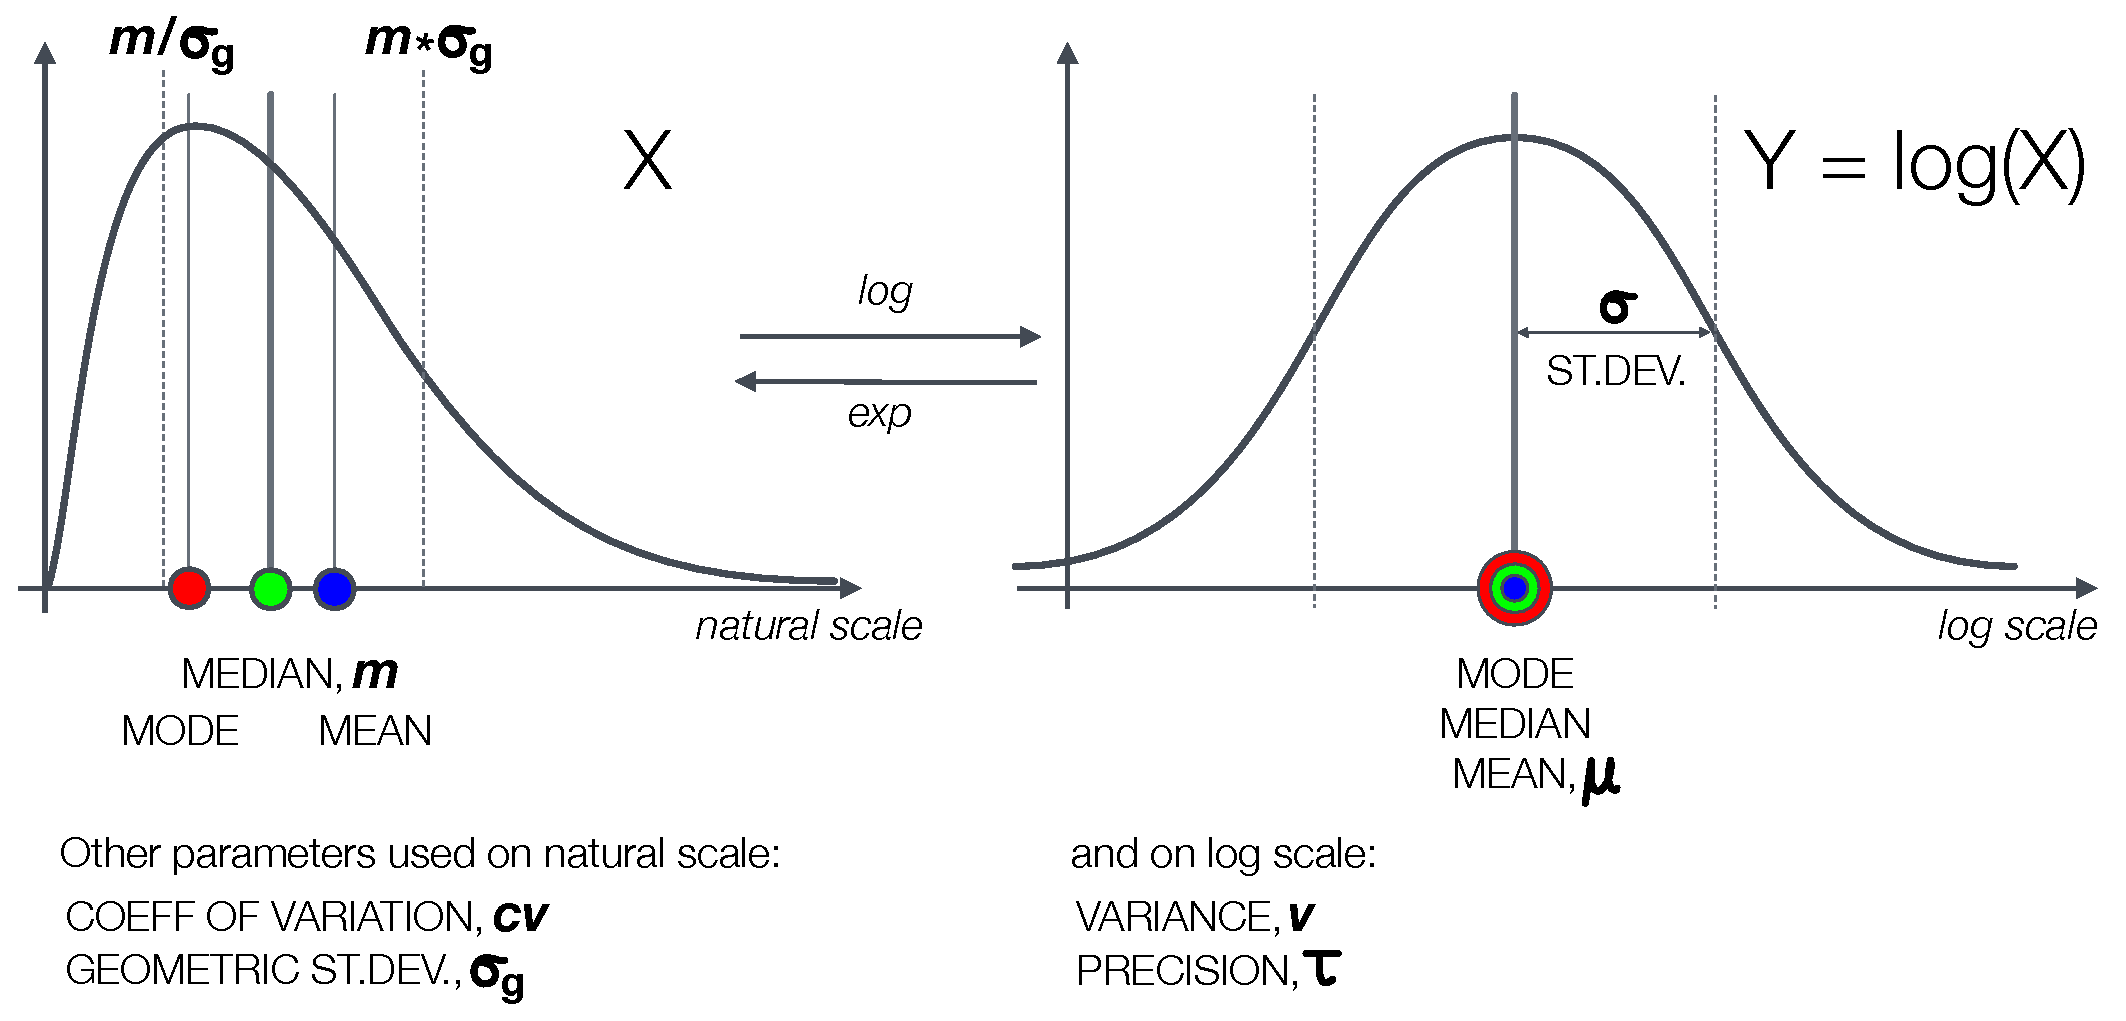
\includegraphics[width=160mm]{pics/LogNormalNormalSchema}
\end{tabular}
\caption{Schematic representation of the lognormaly distributed data on the natural (left) 
and logarithmic scale (right), see Figure \ref{fig:insulinData} for real-life data example. 
\textbf{Bold} symbols stand for quantities commonly used to parameterise a log-normally 
distributed variable.}
\label{fig:schematicLogNormal}
\end{figure}

\subsection{Log-normal distribution}
\label{subsec:logNormalForms}
The log-normal distribution is special in that not only different parameter sets exist
but also because they are defined either on the natural or logarithmic scale. Interestingly, in one 
case the parameters are defined on two different scales, see Figure \ref{fig:schematicLogNormal},
for an overview.\\
Available parameterisations (also listed in Table \ref{figTable:univariates} 
with indication about their coverage in target tools) are 
\begin{itemize}
\item
LogNormal1\,($\mu$, $\sigma$) with \emph{mean}, $\mu$, and \emph{standard deviation}, $\sigma$, both on the log-scale, 
\begin{align*}
P(x;\boldsymbol\mu,\boldsymbol\sigma)= \frac{1}{x \sigma \sqrt{2 \pi}} \exp\Big[ \frac{-(\log x - \mu)^2}{2\sigma^2}\Big]
\end{align*}
\item
LogNormal2\,($\mu$, \textit{v}) with \emph{mean}, $\mu$, and \emph{variance}, $v$, both on the log-scale, 
\begin{align*}
P(x;\boldsymbol\mu,\boldsymbol {v})=\Gape[.5cm][.3cm]{} \frac{1}{x \sqrt{v} \sqrt{2 \pi}} \exp\Big[ \frac{-(\log x - \mu)^2}{2 v}\Big]
\end{align*}
\item
LogNormal3\,(\textit{m}, $\sigma$)  with \emph{median}, $m$, on the natural scale and \emph{standard deviation}, $\sigma$, on the log-scale, 
\begin{align*}
P(x;\boldsymbol m,\boldsymbol \sigma) =\Gape[.5cm][.3cm]{} \frac{1}{x \sigma \sqrt{2 \pi}} \exp\Big[ \frac{-[\log(x/m)]^2}{2\sigma^2}\Big]
\end{align*}
\item
LogNormal4\,(\textit{m}, \textit{cv}) with \emph{median}, $m$, and \emph{coefficient of variation}, $cv$, both on the natural scale, 
\begin{align*}
P(x;\boldsymbol m,\boldsymbol {cv})=\Gape[.5cm][.3cm]{} \frac{1}{x \sqrt{\log(cv^2+1)} \sqrt{2 \pi}} \exp\Big[ \frac{-[\log(x/m)]^2}{2\log(cv^2+1)}\Big]
\end{align*}
\item
LogNormal5\,($\mu$, $\tau$) with \emph{mean}, $\mu$, and \emph{precision}, $\tau$, both on the log-scale.
\begin{align*}
P(x;\boldsymbol\mu,\boldsymbol \tau)=\Gape[.5cm][.3cm]{} \sqrt{\frac{\tau}{2 \pi}} \frac{1}{x} \exp\Big[ {-\frac{\tau}{2}(\log x-\mu)^2} \Big] 
\end{align*}
\item
LogNormal6\,(\textit{m}, $\sigma_g$)  with \emph{median}, $m$, and \emph{geometric st. deviation}, $\sigma_g$, both on the natural scale, \cite{limpert2001log}.
\begin{align*}
P(x;\boldsymbol m,\boldsymbol {\sigma_g})=\Gape[.5cm][.3cm]{} \frac{1}{x \log(\sigma_g)\sqrt{2 \pi}} \exp\Big[ \frac{-[\log(x/m)]^2}{2 \log^2(\sigma_g)}\Big].
\end{align*}
\end{itemize}

Figure \ref{fig:schematicLogNormal} shows the schematic representation of 
lognormaly distributed data on the natural (left) and logarithmic scale (right), 
and indicates, on bold font, the available parameters characterising the 
distribution. On the other hand Figure \ref{fig:insulinData} shows a real-life data 
example. We have used the basal insulin data in diabetic patients \cite{Rudenski:1991aa}.

\begin{figure}[htb!]
\centering
\begin{tabular}{cc}
 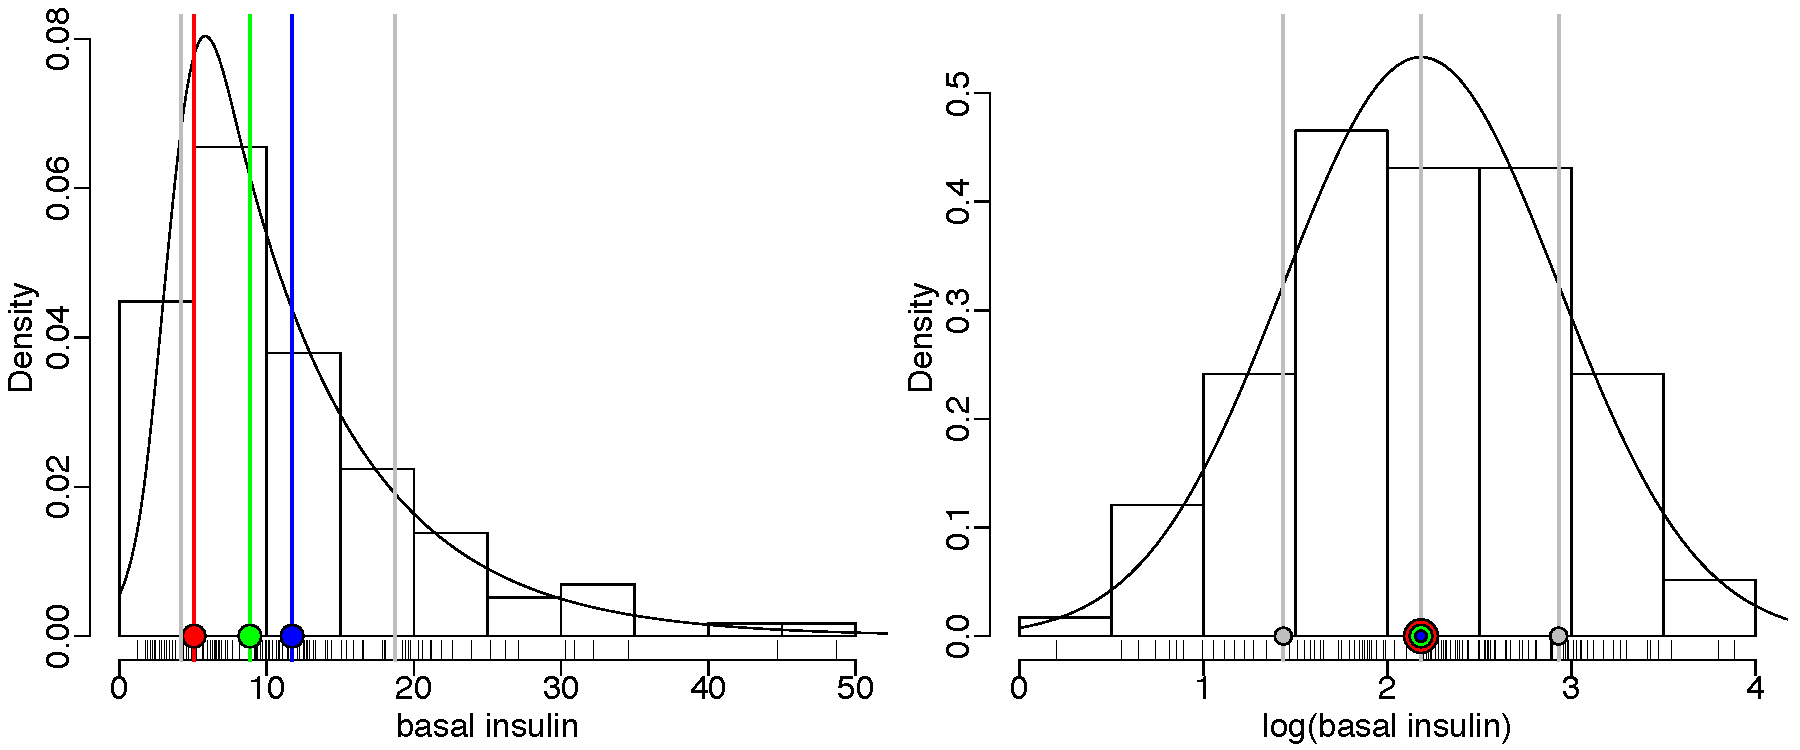
\includegraphics[width=160mm]{pics/Rudenski_LogNormalNormal}
\end{tabular}
\caption{Representation of the lognormaly distributed basal insulin data in diabetic patients 
\cite{Rudenski:1991aa} on the natural scale (left) and on the logarithmic scale after 
$log$--transformation (right), colour code as in Figure \ref{fig:schematicLogNormal}. 
The density estimation for the data on the natural scale and its plotting was performed 
using the R package \textit{logspline} \cite{Kooperberg:2013}. The mode (red) on the 
natural scale doesn't tally with the maximum of the density curve as it should because 
it the latter is an approximation.}
\label{fig:insulinData}
\end{figure}

\subsubsection{Re-parameterisation formulas}
\label{subsubsec:formulas}
The recalculation between given parameterisations is error prone 
and should, whenever required, be taken over by the converters. The 
following equations might be useful when providing such translation support 
between target tools. For example when translating a model implemented 
for Monolix/NONMEM, which use either LN1 or LN2, with winBUGS as the 
target tool, which uses only LN5.\\
\begin{itemize}
%LN1
\item 
LN1 relationships
\begin{itemize}
%LN1
\item 
\begin{description}
\item[LN1($\mu$, $\sigma$) $\rightarrow$ LN2($\mu$, $v$)]:
$\mu \rightarrow \mu; \quad \sigma \rightarrow v=\sigma^2$

\item[LN2($\mu$, $v$) $\rightarrow$ LN1($\mu$, $\sigma$)]:
$\mu \rightarrow \mu; \quad v \rightarrow \sigma = \sqrt{v}$
\end{description}

\item 
\begin{description}
\item[LN1($\mu$, $\sigma$) $\rightarrow$ LN3($m$, $\sigma$)]:
$\mu \rightarrow m=\exp(\mu); \quad \sigma \rightarrow \sigma$

\item[LN3($m$, $\sigma$) $\rightarrow$ LN1($\mu$, $\sigma$)]:
$m \rightarrow \mu=\log(m); \quad \sigma \rightarrow \sigma$
\end{description}

\item 
\begin{description}
\item[LN1($\mu$, $\sigma$) $\rightarrow$ LN4($m$, $cv$)]:
$\mu \rightarrow m=\exp(\mu); \quad \sigma \rightarrow cv=\sqrt{\exp(\sigma^2)-1}$

\item[LN4($m$, $cv$) $\rightarrow$ LN1($\mu$, $\sigma$)]:
$m \rightarrow \mu=\log(m); \quad cv \rightarrow \sigma=\sqrt{\log(cv^2 + 1)}$
\end{description}

\item 
\begin{description}
\item[LN1($\mu$, $\sigma$) $\rightarrow$ LN5($\mu$, $\tau$)]:
$\mu \rightarrow \mu; \quad \sigma \rightarrow \tau=1/\sigma^2$

\item[LN5($\mu$, $\tau$) $\rightarrow$ LN1($\mu$, $\sigma$)]:
$\mu \rightarrow \mu; \quad \tau \rightarrow \sigma=1/\sqrt{\tau}$
\end{description}

\item 
\begin{description}
\item[LN1($\mu$, $\sigma$) $\rightarrow$ LN6($m$, $\sigma_g$)]:
$\mu \rightarrow m=\exp(\mu); \quad \sigma \rightarrow \sigma_g=\exp(\sigma)$

\item[LN6($m$, $\sigma_g$) $\rightarrow$ LN1($\mu$, $\sigma$)]:
$m \rightarrow \mu=\log(m); \quad \sigma_g \rightarrow \sigma=\log(\sigma_g)$
\end{description}
\end{itemize}

%LN2
\item 
remaining LN2 relationships
\begin{itemize}
\item 
\begin{description}
\item[LN2($\mu$, $v$) $\rightarrow$ LN3($m$, $\sigma$)]:
$\mu \rightarrow m=\exp(\mu); \quad v \rightarrow \sigma=\sqrt{v}$

\item[LN3($m$, $\sigma$) $\rightarrow$ LN2($\mu$, $v$)]:
$m \rightarrow \mu=\log(m); \quad \sigma \rightarrow v=\sigma^2$
\end{description}

\item 
\begin{description}
\item[LN2($\mu$, $v$) $\rightarrow$ LN4($m$, $cv$)]:
$\mu \rightarrow m=\exp(\mu); \quad v \rightarrow cv=\sqrt{\exp(v) -1}$

\item[LN4($m$, $cv$) $\rightarrow$ LN2($\mu$, $v$)]:
$m \rightarrow \mu=\log(m); \quad cv \rightarrow v=\log(cv^2+1)$
\end{description}

\item 
\begin{description}
\item[LN2($\mu$, $v$) $\rightarrow$ LN5($\mu$, $\tau$)]:
$\mu \rightarrow \mu; \quad v \rightarrow \tau=1/v$

\item[LN5($\mu$, $\tau$) $\rightarrow$ LN2($\mu$, $v$)]:
$\mu \rightarrow \mu; \quad \tau \rightarrow v=1/\tau$
\end{description}

\item 
\begin{description}
\item[LN2($\mu$, $v$) $\rightarrow$ LN6($m$, $\sigma_g$)]:
$\mu \rightarrow m=\exp(\mu); \quad v \rightarrow \sigma_g=\exp(\sqrt{v})$

\item[LN6($m$, $\sigma_g$) $\rightarrow$ LN2($\mu$, $v$)]:
$m \rightarrow \mu=\log(m); \quad \sigma_g \rightarrow v=\log(\sigma_g^2)$
\end{description}
\end{itemize}

%LN3
\item 
remaining LN3 relationships
\begin{itemize}
\item 
\begin{description}
\item[LN3($m$, $\sigma$) $\rightarrow$ LN4($m$, $cv$)]:
$m \rightarrow m; \quad \sigma \rightarrow cv=\sqrt{\exp(\sigma^2)-1}$

\item[LN4($m$, $cv$) $\rightarrow$ LN3($m$, $\sigma$)]:
$m \rightarrow m; \quad cv \rightarrow \sigma=\sqrt{\log(cv^2 + 1)}$
\end{description}

\item 
\begin{description}
\item[LN3($m$, $\sigma$) $\rightarrow$ LN5($\mu$, $\tau$)]:
$m \rightarrow \mu=\log(m); \quad \sigma \rightarrow \tau=1/\sigma^2$

\item[LN5($\mu$, $\tau$) $\rightarrow$ LN3($m$, $\sigma$)]:
$\mu \rightarrow m=\exp(\mu); \quad \tau \rightarrow \sigma=1/\sqrt{\tau}$
\end{description}

\item 
\begin{description}
\item[LN3($m$, $\sigma$) $\rightarrow$ LN6($m$, $\sigma_g$)]:
$m \rightarrow m; \quad \sigma \rightarrow \sigma_g=\exp(\sigma)$

\item[LN6($m$, $\sigma_g$) $\rightarrow$ LN3($m$, $\sigma$)]:
$m \rightarrow m; \quad \sigma_g \rightarrow \sigma=\log(\sigma)$
\end{description}
\end{itemize}

%LN4
\item 
remaining LN4 relationships
\begin{itemize}
\item 
\begin{description}
\item[LN4($m$, $cv$) $\rightarrow$ LN5($\mu$, $\tau$)]:
$m \rightarrow \mu=\log(m); \quad cv \rightarrow \tau=1/\log(cv^2+1)$

\item[LN5($\mu$, $\tau$) $\rightarrow$ LN4($m$, $cv$)]:
$\mu \rightarrow m = \exp(\mu); \quad \tau \rightarrow cv=\sqrt{\exp(1/\tau)-1}$
\end{description}

\item 
\begin{description}
\item[LN4($m$, $cv$) $\rightarrow$ LN6($m$, $\sigma_g$)]:
$m \rightarrow m; \quad cv \rightarrow \sigma_g=\exp\!\big(\sqrt{\log(cv^2+1)}\big) $%\sqrt{cv+1}$

\item[LN6($m$, $\sigma_g$) $\rightarrow$ LN4($m$, $cv$)]:
$m \rightarrow m; \quad \sigma_g \rightarrow cv=\sqrt{\exp\!\big(\log^2(\sigma_g)\big) -1}$ %\sigma_g^2-1$
\end{description}
\end{itemize}

%LN5
\item 
remaining LN5 relationship
\begin{itemize}\item 
\begin{description}
\item[LN5($\mu$, $\tau$) $\rightarrow$ LN6($m$, $\sigma_g$)]:
$\mu \rightarrow m=\exp(\mu); \quad \tau \rightarrow \sigma_g= \exp(1/\sqrt{\tau})$

\item[LN6($m$, $\sigma_g$) $\rightarrow$ LN5($\mu$, $\tau$)]:
$m \rightarrow \mu=\log(m); \quad \sigma_g \rightarrow \tau= 1/\log^2 (\sigma_g)$
\end{description}
\end{itemize}

\end{itemize}

The proof of the majority of the formulas is straightforward taking into account the definition
of the parameters in question. The relationship between $\sigma$ or $\tau$ (on the log scale) 
and $cv$ (on the natural scale), essential for the re-calculation formulas involving
LN4 parameterisation, is a bit more tricky to see. The 
proof starts with the known relationships for the mean, $mean$, and variance, $var$, on the natural 
scale, collected in table \ref{figTable:logNormalParameterisations}. 
Then the square of the coefficient of variation, $cv$, on the natural scale reads
\begin{align}
	cv^2 &= \frac{var}{mean^2} = \frac{(e^{\sigma^2}-1)\; e^{2\mu + \sigma^2}}{[e^{(\mu + 1/2\sigma^2)}]^2}
	= (e^{\sigma^2}-1) \Leftrightarrow cv = \sqrt{e^{\sigma^2}-1} \;\;\; \& \;\;\; \sigma=\sqrt{\log(cv^2 + 1)}. \nonumber
%	\frac{\cancel{a= b+c}}{\cancel{f} & = b-c
\end{align}
To see then the relationships between $cv$ and $\sigma_g$ on the natural scale 
one has to recall the formula $\sigma_g = exp(\sigma)$, see the 
table \ref{figTable:logNormalParameterisations} and we get the results
\begin{align}
	cv=\sqrt{\exp\!\big(\log^2(\sigma_g)\big) -1} \;\;\; \& \;\;\; \sigma_g=\exp\!\big(\sqrt{\log(cv^2+1)}\big) .\nonumber
%	\frac{\cancel{a= b+c}}{\cancel{f} & = b-c
\end{align}

\begin{figure}[htb!]
\centering
 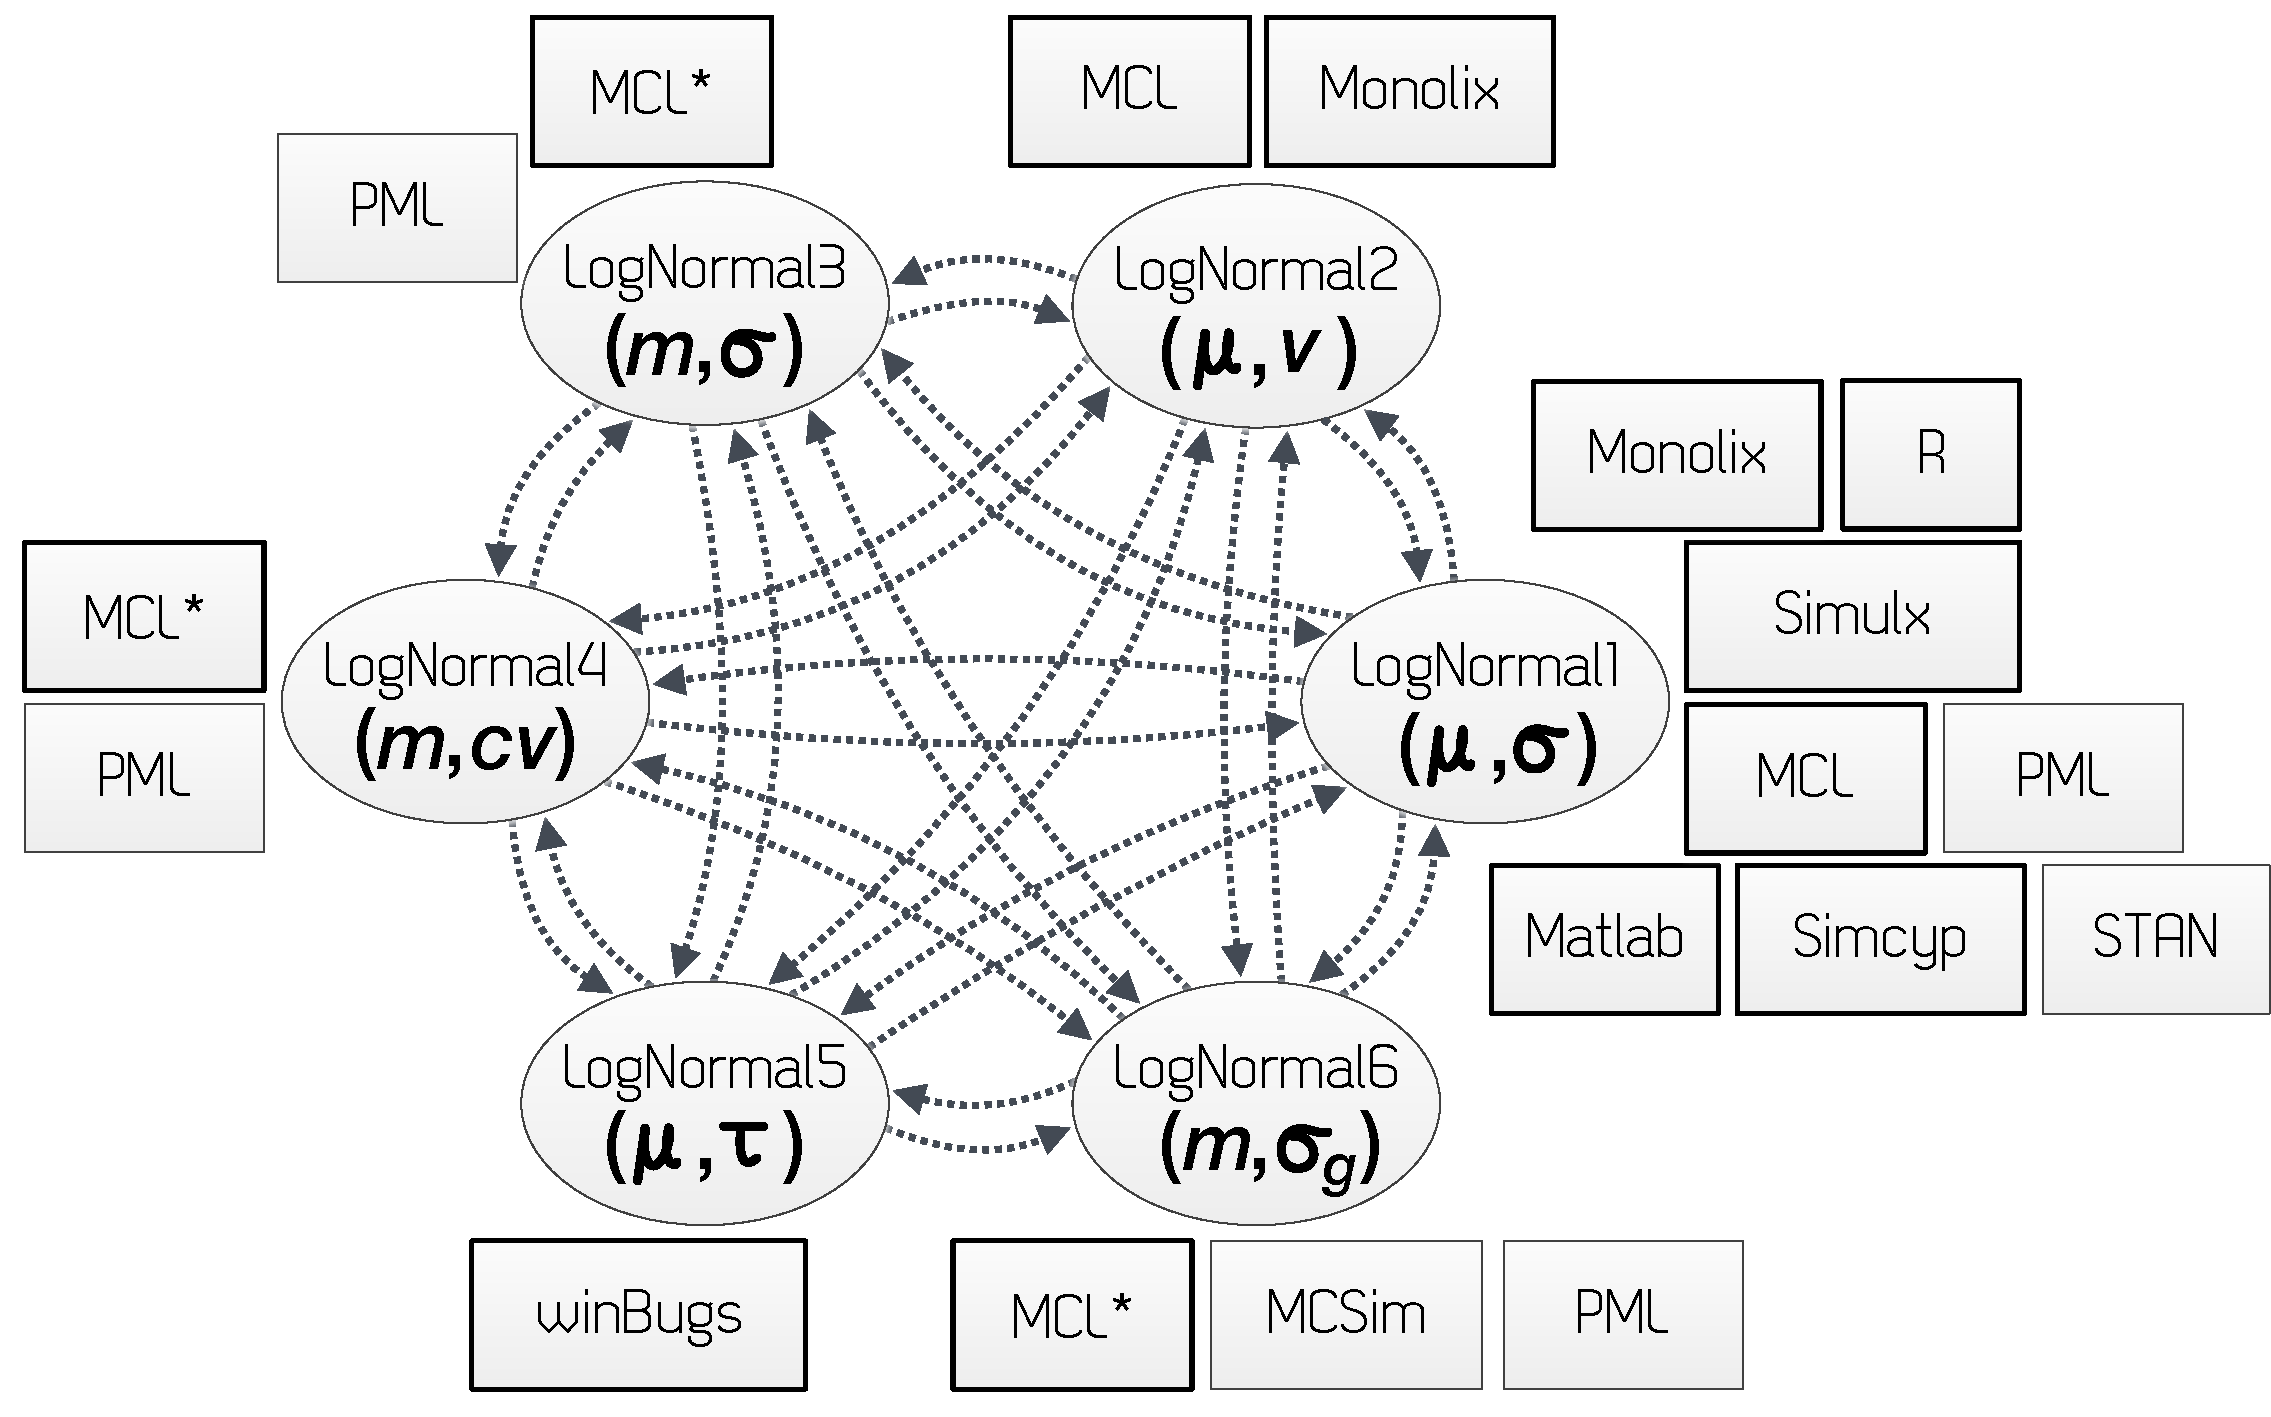
\includegraphics[width=145mm]{pics/LNreparams}
\caption{Re-parameterisation relationships implemented in ProbOnto and their support 
in target (black edges) and few selected other languages/tools. * Indication of the 
planned support for the according parameterisations in MCL.}
\label{fig:LNreparams}
\end{figure}

%\footnote{Based on a Stack Overflow discussion \url{tinyurl.com/qavgvln}}
%\newpage
\subsubsection{Overview table}

%\cleardoublepage
\setlength{\tabcolsep}{1.5em}
\captionsetup[longtable]{skip=1em}
\LTcapwidth=.95\textwidth
\begin{center}
\small
\renewcommand{\arraystretch}{1}%
\begin{longtable}{ccc}
 \hline
 \hline
\multicolumn{1}{c}{Log-normal distribution} 	& \multirow{2}{*}{Quantity} 	&\multicolumn{1}{c}{Normal distribution on the} \\ [-.5ex]
\multicolumn{1}{c}{on the natural scale (NS)} 	&						& \multicolumn{1}{c}{log-transformed scale (LS)} \\
   \hline
  \hline
  \multicolumn{3}{c}{\Gape[.3cm][.1cm]{}$LN1(\boldsymbol\mu,\boldsymbol\sigma) =\frac{1}{x \sigma \sqrt{2 \pi}} \exp\Big[ \frac{-(\log x - \mu)^2}{2\sigma^2}\Big] $ }\\
   \hline
$e^{\mu + \frac{1}{2}\sigma^2}$			& \Gape[.4cm][0cm]{}Mean  	& $\boldsymbol\mu$ \\ [.25ex]
$e^{2\mu + \sigma^2}[e^{\sigma^2}-1]$		& Variance 				& $\sigma^2$	\\ [.25ex]
$e^{\mu + \frac{1}{2}\sigma^2}\sqrt{e^{\sigma^2}-1}$ & Standard deviation	& $\boldsymbol\sigma$	\\ [.25ex]
%									& deviation  				&		 	\\ [.25ex]
 $e^{\mu - \sigma^2}$	 				& Mode 					&	 $\mu$	\\ [.25ex]
$e^\mu$								& Median					& $\mu$ \\ [.25ex]
$\sqrt{e^{\sigma^2}-1}$					& Coefficient of variation		& $\sigma/\mu$ \\ [.5EX]
%									& of variation				& \\
  \hline
  \multicolumn{3}{c}{\Gape[.3cm][.1cm]{}$LN2(\boldsymbol\mu,\boldsymbol {v}) = \frac{1}{x \sqrt{v} \sqrt{2 \pi}} \exp\Big[ \frac{-(\log x - \mu)^2}{2 v}\Big] $ }\\
   \hline
$e^{\mu + \frac{1}{2}v}$					& \Gape[.4cm][0cm]{}Mean  	& $\boldsymbol\mu$ \\ [.25ex]
$e^{2\mu + v}[e^{v}-1]$					& Variance 				& $\boldsymbol v$	\\ [.25ex]
$e^{\mu + \frac{1}{2} v}\sqrt{e^{v}-1}$ 		& Standard deviation		& $ {\sqrt{v}}$	\\ [.25ex]
%									& deviation  				& 	\\ [.25ex]
$e^{\mu - v}$	 						& Mode 					& $\mu$	\\ [.25ex]
$e^\mu$								& Median					& $\mu$ \\ [.25ex]
$\sqrt{e^{v}-1}$						& Coefficient of variation		& ${\sqrt{v}} /\mu$ \\ [.5EX]
%									& of variation				& \\
  \hline
  \multicolumn{3}{c}{\Gape[.3cm][.1cm]{}$LN3P(\boldsymbol m,\boldsymbol \sigma)=	 \frac{1}{x \sigma \sqrt{2 \pi}} \exp\Big[ \frac{-[\log(x/m)]^2}{2\sigma^2}\Big] $ }\\ %[1.5EX]
   \hline
 $m\, e^{\frac{1}{2}\sigma^2}$				& \Gape[.4cm][0cm]{}Mean  	& $\log( m)$ \\ [.25ex]
 $m^2 e^{\sigma^2} [e^{\sigma^2}-1]$		& Variance 				& $\sigma^2$	\\ [.25ex]
$m\sqrt{e^{\sigma^2} (e^{\sigma^2}-1)}$		& Standard deviation	  	& $\boldsymbol\sigma$	\\ [.25ex]
%									& deviation  				& 	\\ [.25ex]
 $m/e^{\sigma^2}$	 					& Mode 					& $\log( m)$	\\ [.25ex]
 $\boldsymbol m$						& Median 					& $\log( m)$	\\ [.25ex]
$\sqrt{e^{\sigma^2}-1}$					& Coefficient of variation		& $\sigma/\log( m)$ \\ [.5EX]
% 									&  of variation				&  \\
  \hline
   \multicolumn{3}{c}{\Gape[.3cm][.1cm]{}$LN4(\boldsymbol m,\boldsymbol {cv})= \frac{1}{x \sqrt{\log(cv^2+1)} \sqrt{2 \pi}} \exp\Big[ \frac{-[\log(x/m)]^2}{2\log(cv^2+1)}\Big] $} 	\\
   \hline
 $m \sqrt{cv^2 + 1}$						& \Gape[.4cm][0cm]{}Mean  	& $\log( m)$ \\ [.25ex]
 $m^2 \,(cv^2+1)\,cv^2$					& Variance 				& $\log(cv^2 + 1)$	\\ [.25ex]
$m\,cv \sqrt{(cv^2+1)}$					& Standard  deviation		& $\sqrt{\log(cv^2 + 1)}$	\\ [.25ex]
% 									& deviation  				& 	\\ [.25ex]
 $m / (cv^2 + 1)$	 					& Mode 					& $\log( m)$	\\ [.25ex]
 $\boldsymbol m$						& Median 					& $\log( m)$	\\ [.25ex]
 ${\boldsymbol {cv}}$					& Coefficient of variation		& $\sqrt{\log(cv^2 + 1)}/\log( m)$ \\ [.5EX]
  \hline
  \multicolumn{3}{c}{\Gape[.3cm][.1cm]{}$LN5(\boldsymbol\mu,\boldsymbol \tau)= \sqrt{\frac{\tau}{2 \pi}} \frac{1}{x} \exp\Big[ {-\frac{\tau}{2}(\log x-\mu)^2} \Big] $ }\\
   \hline
 $e^{\mu + \frac{1}{2\tau}}$							& \Gape[.4cm][0cm]{}Mean  	& $\boldsymbol\mu$ \\ [0ex]
 $e^{2\mu + \frac{1}{\tau}}[e^{\frac{1}{\tau}}-1]$ 			& Variance 				& $1/\tau$	\\ [0ex]
$e^{\mu + \frac{1}{2} \frac{1}{\tau}}\sqrt{e^{\frac{1}{\tau}}-1}$ 	& Standard deviation 		& $\sqrt{1/\tau}$	\\ [0ex]
 $e^{\mu - \frac{1}{\tau}}$								& Mode 					& $\mu$	\\ [0ex]
 $e^\mu$											& Median					& $\mu$ \\ [0ex]
$\sqrt{e^{\frac{1}{\tau}}-1}$							& Coefficient of variation		& $\sqrt{1/\tau} / \mu$ \\ [0EX]
  $1/\big(e^{2\mu + \frac{1}{\tau}}[e^{\frac{1}{\tau}}-1]\big)$ 	& Precision				& $\boldsymbol\tau$ \\ [0ex]
  \hline
  \multicolumn{3}{c}{\Gape[.3cm][.1cm]{}$LN6(\boldsymbol m,\boldsymbol {\sigma_g})= \frac{1}{x \log(\sigma_g)\sqrt{2 \pi}} \exp\Big[ \frac{-[\log(x/m)]^2}{2 \log^2(\sigma_g)}\Big] $ }\\
   \hline
% $m \exp(\frac{1}{2} \log^2(\sigma_g))$						& \Gape[.4cm][0cm]{}Mean  	& $\log( m)$ \\ [.25ex]
 $m\,e^{\frac{1}{2} \log^2(\sigma_g)}$						& \Gape[.4cm][0cm]{}Mean  	& $\log( m)$ \\ [.25ex]
% $m^2 \exp(\log^2(\sigma_g))[\exp(\log^2(\sigma_g))-1]$		& Variance 				& $\log(\sigma_g^2)$	\\ [.25ex]
 $\sigma_g^2$											& Variance 				& $\log^2(\sigma_g)$	\\ [.25ex]
%$\sqrt{m^2 \exp(\log^2(\sigma_g))[\exp(\log^2(\sigma_g))-1]}$ 	& Standard  deviation		& $\log(\sigma_g)$	\\ [.25ex]
$\boldsymbol {\sigma_g}$ 								& Standard  deviation		& $\log(\sigma_g)$	\\ [.25ex]
% $m / \exp(\log^2(\sigma_g))$	 						& Mode 					& $\log( m)$	\\ [.25ex]
 $m / e^{\log^2(\sigma_g)}$	 							& Mode 					& $\log( m)$	\\ [.25ex]
 $\boldsymbol m$										& Median 					& $\log( m)$	\\ [.25ex]
% $\sqrt{\exp(\log^2(\sigma_g))-1}$							& Coefficient of variation		& $-$ \\ [.5EX]
 $\sigma_g / (m\, e^{\frac{1}{2} \log^2(\sigma_g)})$				& Coefficient of variation		& $\log(\sigma_g)/\log( m)$ \\ [.5EX]
   \hline
\caption{The available parameterisations for the log-normal distribution and their characterising 
quantities as functions of the respective parameters. With $\boldsymbol m$ -- median (NS), 
$\boldsymbol {cv}$ -- coefficient of variation (NS), $\boldsymbol \mu$ -- mean (LS), 
$\boldsymbol \sigma$ -- standard deviation (LS), $\boldsymbol \sigma_g$ -- geometric standard 
deviation (NS), $\boldsymbol v$ -- variance (LS), 
$\boldsymbol \tau$ -- precision (LS). See Figure \ref{fig:schematicLogNormal} and 
section \ref{subsec:logNormalForms} for the meaning of the symbols.
%\\ \small Small print: 
%The re-parameterisation formulas, page \pageref{subsubsec:formulas}, and expressions in this table are partially from 
%literature, partially self calculated (by MJS), use them on your own risk.
%Results for LN2 on the left identical with those on Vose's page.
%Median and variance for LN3 on the left identical to Leemis.
}
\label{figTable:logNormalParameterisations}
\vspace{-2.5em}
\end{longtable}
\end{center}

%\newpage 
\section{Distributions in ProbOnto}
\subsection{Univariates -- ProbOnto and tool coverage}
\captionsetup[longtable]{skip=1em}
\LTcapwidth=.95\textwidth
\begin{center}
\setlength{\tabcolsep}{7pt}
%\small
\renewcommand{\arraystretch}{1.1}%
\begin{longtable}{l | lcccc}
  \hline
  \hline
\multicolumn{1}{c}{\textbf{ProbOnto}}& Parameters 	& \textbf{UncertML} 	& \textbf{WinBUGS}	& \textbf{Monolix} 	& \textbf{NONMEM} \\
\multicolumn{1}{c}{0.3}			&			&  3.0			& 1.4			& 4.3			& 7.3 \\
  \hline
  \hline
  \multicolumn{6}{c}{\textit{Discrete Univariate}}  \\
  \hline
Bernoulli				& \emph{p}		& y	& y	& --  &  -- \\
Binomial				& \emph{n, p}		& y	& y	& --  &  -- \\
Categorical ordered		& $p_1, \ldots, p_k$	& y	& y	& --  &  -- \\
Categorical unordered	& $p_1, \ldots, p_k$	& y	& y	& --  &  -- \\
DoublePoisson1		& $\mu, \phi$		& --	& --	& --  &  -- \\
Generalized Poisson 1	& $\theta, \delta$	& --  	& --  & --  &  -- \\
Generalized Poisson 2	& $\mu, \delta$		& --  	& --  & --  &  -- \\
Generalized Poisson 3	& $\mu, \alpha$	& --  	& --  & --  &  -- \\
Geometric			& \emph{p}		& y	& --  & --  &  -- \\
Hypergeometric		& \emph{N, K, n}	& y	& --  & --  &  -- \\
Inverse Binomial 		& $k, p$ 			& --  	& --  & --  &  -- \\
Negative Binomial 1		& \emph{r, p}		& --	& y	& --  &  -- \\
Negative Binomial 2 		& $\lambda, \tau$ 	& --  	& --  & --  &  -- \\
Negative Binomial 3 		& $\mu, k$ 		& --  	& --  & --  &  -- \\
Negative Binomial 4 		& $r,p$ 			& y  	& --  & --  &  -- \\
Poisson				& $\lambda$		& y	& y	& --  &  -- \\
Uniform Discrete 1 		&  \emph{a, b, n}	& --	& --	& -- & --  \\
Uniform Discrete 2 		&  $a=0$, \emph{n}	& --	& --	& -- & --  \\
Zero-Inflated Negative Binomial & $\lambda, \tau, p0$	& --  & --  & --  &  -- \\
Zero-Inflated Poisson	& $\lambda, \pi$	& --  & --  & --  &  -- \\
  \hline
  \multicolumn{6}{c}{\textit{Continuous Univariate}}	\\
  \hline
Beta					& $\alpha, \beta$	& y	& y	& y	&  -- \\
Birnbaum-Saunders		& $\alpha, \gamma$	& --	& --	& --	&  -- \\
Cauchy				& $x_0, \gamma$	& y	& --  & --  &  -- \\
Chi-squared			& \emph{k}		& y	& y	& y	&  -- \\
%Dirac Delta			&	&	y	& --  & --  &  -- \\
Exponential			& $\lambda$		& y	& y	& y	&  -- \\
F (aka Fisher-Snedecor)	& $d_1, d_2$		& y	& --  & y	&  -- \\
Gamma				& $k, \theta$		& y	& y	& y	&  -- \\
Generalized Gamma 1	& \emph{a, d, p}	& --	& --  & --  & --  \\
Generalized Gamma 2	& \emph{a, b, c, k}	& --	& --  & --  & --  \\
Gompertz				& $\eta, b$		& --  & y	& --  & --  \\
Gumbel (aka Extreme Value)	& $\mu, \beta$	& --  & y 	& --  & -- \\ 
Inverse-Gamma		& $\alpha, \beta$	& y	& --  & --  &  -- \\
Inverse-Gaussian (aka Wald)	& $\lambda, \mu$	& --	& --  & --  &  -- \\
Laplace 1				& \multirow{2}{*}{$\mu, b$} &	\multirow{2}{*}{y}	&	\multirow{2}{*}{--}	& \multirow{2}{*}{--}  & \multirow{2}{*}{--} \\ 
(aka Double-exponential) \\
Laplace 2				& $\mu, \tau$ 		&	--	&	y	& --  & -- \\ 
Logistic				& $\mu, s$		&	y	&	y	& --  &  -- \\
Log-Logistic (aka Fisk)	& $\alpha, \beta$		&	y	&	y	& --  &  -- \\
Log-Normal 1			& $\mu, \sigma$	&	y	&	--	&	y	&  -- \\
Log-Normal 2			& $\mu$, \textit{v}	&	y	&	--	&	y	&  -- \\
Log-Normal 3			& \emph{m}, $\sigma$	&	--	&	--	&	--	&  -- \\
Log-Normal 4			& \emph{m, cv}		& 	--	&	--	&	--	&  -- \\
Log-Normal 5			& $\mu$, $\tau$	& 	--	&	y	&	--	&  -- \\
Log-Normal 6			& $m$, $\sigma_g$	& 	--	&	--	&	--	&  -- \\
Log-Uniform			& $min$, $max$	& 	--	&	--	&	--	&  -- \\
Nakagami				& $m, \Omega$	&	--	&	--	&	--	&  --  \\
Normal 1				& $\mu, \sigma$	&	y	&	--	&	y	& y  \\
Normal 2				& $\mu, v$		&	y	&	--	&	y	&  -- \\
Normal 3				& $\mu, \tau$		&	--	&	y	&	--	&  -- \\
Normal-inverse-gamma	& $\mu, \lambda, \alpha, \beta$	& y	& --  & --  &  -- \\
Pareto				& $x_m, \alpha$	& y	& y	& --  &  -- \\
Rayleigh				& $\sigma$		& --  & --  & y	&  -- \\
Standard Normal 		& $\mu\!=\!0, \sigma\!=\!1$	& y & -- &	 y & y  \\
Standard Uniform		& $a\!=\!0, b\!=\!1$		& --	& --	& y & y  \\
Student's T			& $\nu$			& y	& y	& y	&  -- \\
Triangular				& $a, b, c$		& -- 	& --	& -- & -- \\
TruncatedNormal		& $\mu, \sigma, a, b$ & --	& --  & -- & -- \\
Uniform				&  \emph{a, b}		& y	& y	& y		& --  \\
Weibull 1				& $\lambda, k$		& y	& --	& y	&  -- \\
Weibull 2				& $\lambda, v$		& --	& y	& --	&  -- \\
   \hline 
\caption{{\color{red} \scshape{updated}} Univariate distributions supported in ProbOnto with overview of tool support. 
See Appendix \ref{ch:probontoAppendix} for a detailed description of each distribution.}
\label{figTable:univariates}
\vspace{-2.5em}
\end{longtable}
\end{center}

\subsection{Univariates -- code names}
\captionsetup[longtable]{skip=1em}
\LTcapwidth=.95\textwidth
\begin{center}
\setlength{\tabcolsep}{7pt}
%\small
\renewcommand{\arraystretch}{1.1}%
\begin{longtable}{l | llllll}
  \hline
  \hline
\multicolumn{1}{c}{\textbf{Distribution}}& \multicolumn{6}{c}{\textbf{Parameters}} \\ 
Code name		& Symbol & Code name & Symbol & Code name \\
  \hline
  \hline
  \multicolumn{6}{c}{\textit{Discrete Univariate}}  \\
  \hline
\xatt{Bernoulli1}			& \emph{p}		& \xatt{probability} 		& --			& -- \\
\xatt{Binomial1} 			& \emph{n}		& \xatt{numberOfTrials}& \emph{p}	& \xatt{probability} \\
\xatt{CategoricalOrdered1}	& $p_1,\dots,p_k$ 	& \xatt{categoryProb}  	&  --			& -- \\
\xatt{CategoricalUnordered1}	& $p_1,\dots ,p_k$ 	& \xatt{categoryProb}	&  --			& -- \\
\xatt{DoublePoisson1}		& $\mu$			& \xatt{rate}			& $\phi$		& \xatt{dispersion} \\
\xatt{GeneralizedPoisson1}	& $\theta$			& \xatt{rate}			& $\delta$		& \xatt{dispersion} \\
\xatt{GeneralizedPoisson2}	& $\mu$			& \xatt{mean}			& $\delta$		& \xatt{dispersion} \\
\xatt{GeneralizedPoisson3}	& $\mu$			& \xatt{mean}			& $\alpha$	& \xatt{dispersion} \\
\xatt{Geometric1} 			& \emph{p}		& \xatt{probability}		& --			& --	\\
\xatt{Hypergeometric1} 		& \emph{N}		& \xatt{populationSize}	& \emph{K}	& \xatt{numberOfSuccesses} \\[-0.5ex]
						&				&					&\emph{n}	& \xatt{numberOfTrials} \\
\xatt{InverseBinomial1} 		& $k$ 			& \xatt{index}			& $p$		& \xatt{probability}	\\
\xatt{NegativeBinomial1} 		& \emph{r}		& \xatt{numberOfSuccesses}&  \emph{p}	& \xatt{probability}	\\
\xatt{NegativeBinomial2} 		& $\lambda$ 		& \xatt{rate}			& $\tau$		& \xatt{overdispersion}	\\
\xatt{NegativeBinomial3} 		& $\mu$ 			& \xatt{mean}			& $k$		& \xatt{index}	\\
\xatt{NegativeBinomial4} 		& $r$ 			& \xatt{numberOfFailures}& $p$		& \xatt{probability}	\\
\xatt{Poisson1}				& $\lambda$		& \xatt{rate}			& --			& -- 	\\
\xatt{UniformDiscrete1} 		&  \emph{a}		& \xatt{minimum}		& \emph{b}	& \xatt{maximum}	\\[-0.5ex]
						&				&					& \emph{n} 	& \xatt{numberOfValues} \\
\xatt{UniformDiscrete2} 		& $a=0$			& \xatt{minimum}		& \emph{n} 	& \xatt{numberOfValues}	\\
\xatt{ZeroInflatedNegativeBinomial1} & $\lambda$	& \xatt{rate}			& $\tau$ 		& \xatt{overdispersion}	\\
						&				&					& $p0$		& \xatt{probabilityOfZero} \\
\xatt{ZeroInflatedPoisson1} 	& $\lambda$		& \xatt{rate}			& $\pi$ 		& \xatt{probabilityOfZero}	\\
  \hline
  \multicolumn{7}{c}{\textit{Continuous Univariate}}	\\
  \hline
\xatt{Beta1} 				& $\alpha$		& \xatt{alpha}			& $\beta$		& \xatt{beta}		\\
\xatt{BirnbaumSaunders1}	& $\alpha$		& \xatt{scale}			& $\gamma$	& \xatt{shape}		\\
\xatt{Cauchy1} 				& $x_0$			& \xatt{location}		& $\gamma$	& \xatt{scale}		\\
\xatt{ChiSquared1}			& \emph{k}		& \xatt{degreesOfFreedom} & --		&  --				\\
\xatt{Exponential1}			& $\lambda$		& \xatt{rate}			& --			& -- 				\\
\xatt{F1}					& $d_1$			& \xatt{numerator}		& $d_2$		& \xatt{denominator} \\
\xatt{Gamma1}				& $k$			& \xatt{shape}			& $\theta$	& \xatt{scale} 			\\
\xatt{GeneralizedGamma1}	& \emph{a}		& \xatt{scale}			& \emph{d}	& \xatt{shape1}		\\
						& 				& 					& \emph{k} 	& \xatt{shape2} 	\\
\xatt{GeneralizedGamma2}	& \emph{a}		& \xatt{location}		& \emph{b}	& \xatt{scale}		\\
						& \emph{c}		& \xatt{shape1} 		& \emph{p} 	& \xatt{shape2} 	\\
\xatt{Gompertz1}			& $\eta$			& \xatt{shape}			& \emph{b}	& \xatt{scale}		\\
\xatt{Gumbel1} 			& $\mu$			& \xatt{location}		& $\beta$		& \xatt{scale}		\\ 
\xatt{InverseGamma1}		& $\alpha$		& \xatt{shape}			& $\beta$		& \xatt{scale}		\\
\xatt{InverseGaussian1}		& $\lambda$		& \xatt{shape}			& $\mu$		& \xatt{mean}		\\
\xatt{Laplace1}				& $\mu$ 			& \xatt{location}		& \emph{b}	& \xatt{scale}		\\
\xatt{Laplace2}				& $\mu$ 			& \xatt{location}		& $\tau$		& \xatt{tau}		\\
\xatt{Logistic1}				& $\mu$			& \xatt{location}		& \emph{s}	& \xatt{scale}		\\
\xatt{LogLogistic1}			& $\alpha$		& \xatt{scale}			& $\beta$		& \xatt{shape}		\\
\xatt{LogNormal1}			& $\mu$			& \xatt{meanLog}		& $\sigma$ 	& \xatt{stdevLog}	\\
\xatt{LogNormal2}			& $\mu$			& \xatt{meanLog}		& \textit{v}		& \xatt{varLog}		\\
\xatt{LogNormal3}			& \emph{m} 		& \xatt{median}			& $\sigma$	& \xatt{stdevLog}	\\
\xatt{LogNormal4}			& \emph{m}		& \xatt{median}			& \emph{cv}	& \xatt{coefVar	}	\\
\xatt{LogNormal5}			& $\mu$			& \xatt{meanLog}		& $\tau$		& \xatt{precision}	\\
\xatt{LogNormal6}			& $m$			& \xatt{median}			& $\sigma_g$	& \xatt{geomStdev}	\\
\xatt{LogUniform1}			& $min$			& \xatt{minimum}		& $max$		& \xatt{maximum}	\\
\xatt{Nakagami1}			& $m$			& \xatt{shape}			& $\Omega$ 	& \xatt{spread}		\\
\xatt{Normal1}				& $\mu$			& \xatt{mean}			& $\sigma$ 	& \xatt{stdev}		\\
\xatt{Normal2}				& $\mu$			& \xatt{mean}			& \emph{v}	& \xatt{var}		\\
\xatt{Normal3}				& $\mu$			& \xatt{mean}			& $\tau$ 		& \xatt{precision} 	\\
\xatt{NormalInverseGamma1}	& $\mu$			& \xatt{mean}			& $\lambda$	& \xatt{lambda}		\\[-0.5ex]
						& $\alpha$ 		& \xatt{alpha}			& $\beta$ 		& \xatt{beta} 		\\
\xatt{Pareto1}				& $x_m$			& \xatt{scale}			& $\alpha$ 	& \xatt{shape} 		\\
\xatt{Rayleigh1}			& $\sigma$		& \xatt{scale}			& --			& -- 				\\
\xatt{StandardNormal1} 		& $\mu\!=\!0$		& \xatt{mean}			& $\sigma\!=\!1$ & \xatt{stdev} 		\\
\xatt{StandardUniform1}		& $a\!=\!0$		& \xatt{minimum}		& $b\!=\!1$ 	& \xatt{maximum}	\\
\xatt{StudentT1}			& $\nu$			& \xatt{degreesOfFreedom} & --		& -- 				\\
\xatt{Triangular1}			& $a$			& \xatt{lowerLimit}		& $b$ 		& \xatt{upperLimit}	\\[-0.5ex]
						&				&					& $c$		& \xatt{shape} 		\\
\xatt{TruncatedNormal1}		& $\mu$			& \xatt{mean}			& $\sigma$ 	& \xatt{stdev}		\\[-0.5ex]
						& $a$			& \xatt{lowerBound}		& $b$		& \xatt{upperBound} \\
\xatt{Uniform1}				& \emph{a}		& \xatt{minimum}		& \emph{b}	& \xatt{maximum}	\\
\xatt{Weibull1}				& $\lambda$		& \xatt{scale}			& \emph{k}	& \xatt{shape}		\\
\xatt{Weibull2}				& $\lambda$		& \xatt{lambda}			& \emph{v}	& \xatt{shape}		\\
   \hline 
\caption{{\color{red} \scshape{updated}} Code names for distribution and parameter names of the univariate distributions.}
\label{figTable:univariatesCodes}
\vspace{-2.5em}
\end{longtable}
\end{center}

%\newpage
\subsection{Multivariates -- ProbOnto and tool coverage}

\captionsetup[longtable]{skip=1em}
\LTcapwidth=.95\textwidth
\begin{center}
\setlength{\tabcolsep}{7pt}
%\small
\renewcommand{\arraystretch}{1.1}%
\begin{longtable}{l | lcccc}
  \hline
  \hline
\multicolumn{1}{c}{\textbf{ProbOnto}} & Parameters & \textbf{UncertML} & \textbf{WinBUGS} & \textbf{Monolix} & \textbf{NONMEM}\\
\multicolumn{1}{c}{0.3}			& 			&  3.0			& 1.4 			& 4.3  		    &	7.3 \\
  \hline
  \hline
  \multicolumn{6}{c}{\textit{Discrete Multivariate}} \\
  \hline
Multinomial	 		& $n, p_1, \ldots, p_k$ 		& y	& y 	& --	& -- 	\\
  \hline
  \multicolumn{6}{c}{\textit{Continuous Multivariate}} \\
  \hline
Dirichlet				& $\alpha_1, \dots, \alpha_K$	& y	& y 	& --	& -- 	\\
Inverse-Wishart		& $\Psi, \nu$				& --  	& --  	& --	& y 	\\[0.5ex]
Multivariate Normal	1 	& $\mu, \Sigma $			& y	& --	& --	& -- 	\\
Multivariate Normal	2 	& $\mu, T $				& --	& y	& --	& -- 	\\[0.5ex]
Multivariate (Student) T 1	& $\mu, \Sigma, \nu$		& y	& --	& --	& -- 	\\
Multivariate (Student) T 2& $\mu, T, k$ 				& --	& y	& --	& -- 	\\[0.5ex]
Wishart 1				& $V, n$					& y	& --	& --	& --  	\\
Wishart 2				& $R, k$					& --	& y	& --	& -- 	\\
   \hline
\caption{Multivariate distributions with overview of tool support. See the Appendix \ref{ch:probontoAppendix}
for the detailed description of each distribution.}
\label{figTable:multivariates}
\vspace{-2.5em}
\end{longtable}
\end{center}

\subsection{Multivariates -- code names}

\captionsetup[longtable]{skip=1em}
\LTcapwidth=.95\textwidth
\begin{center}
\setlength{\tabcolsep}{7pt}
%\small
\renewcommand{\arraystretch}{1.1}%
\begin{longtable}{l | llllll}
  \hline
  \hline
\multicolumn{1}{c}{\textbf{Distribution}}& \multicolumn{4}{c}{\textbf{Parameters}} \\ 
Code name				& Symbol & Code name 			& Symbol 			& Code name \\
  \hline
  \hline
  \multicolumn{5}{c}{\textit{Discrete Multivariate}} \\
  \hline
\xatt{Multinomial1} 			& $n$	& \xatt{numberOfTrials} 	& $p_1, \ldots, p_k$	& \xatt{probabilityOfSuccess}   \\
  \hline
  \multicolumn{5}{c}{\textit{Continuous Multivariate}} \\
  \hline
\xatt{Dirichlet1}				& $\alpha_1, \dots, \alpha_K$	& \xatt{concentration} 	& --		& --  \\
\xatt{InverseWishart1}		& $\Psi$		& \xatt{scaleMatrix}	& $\nu$ 			& \xatt{degreesOfFreedom} \\
\xatt{MultivariateNormal1}	& ${\mu}$		& \xatt{mean}		& $\Sigma$		& \xatt{covarianceMatrix}  \\
\xatt{MultivariateNormal2	}	& ${\mu}$		& \xatt{mean}		& $T$ 			& \xatt{precisionMatrix}	 \\ [0.5ex]
\xatt{MultivariateStudentT1}	& ${\mu}$		& \xatt{mean}		& $\Sigma$		& \xatt{covarianceMatrix} \\[-0.5ex]
						&			&				& $ \nu$			& \xatt{degreesOfFreedom} \\ [0.5ex]
\xatt{MultivariateStudentT2}	& ${\mu}$ 	& \xatt{mean} 		& $T$			& \xatt{precisionMatrix}	 \\[-0.5ex]
						&			&				& $k$ 			& \xatt{degreesOfFreedom} \\
\xatt{Wishart1} 				& $V$		& \xatt{scaleMatrix}	& $n$			& \xatt{degreesOfFreedom} \\
\xatt{Wishart2} 				& $R$		& \xatt{inverseScaleMatrix} & $k$		& \xatt{degreesOfFreedom} \\
   \hline
\caption{Code names for the multivariate distributions and their parameters.}
\label{figTable:multivariatesCodes}
\vspace{-2.5em}
\end{longtable}
\end{center}

\subsection{Mixture distribution}
Because only the mixture distribution for univariate distributions is supported,
we skip one table. Apart from Pronto, the mixture distribution is supported only by UncertML. 

\captionsetup[longtable]{skip=1em}
\LTcapwidth=.95\textwidth
\begin{center}
\setlength{\tabcolsep}{10pt}
%\small
\renewcommand{\arraystretch}{1.1}%
\begin{longtable}{l | cccc}
  \hline
  \hline
\multicolumn{1}{c}{\textbf{ProbOnto}}	&   \multicolumn{2}{c}{Parameters} 	& \textbf{UncertML}  \\
\multicolumn{1}{c}{0.3}				&  Symbol					& Code name 	&  3.0		 \\
  \hline
  \hline
\xatt{MixtureDistribution1} & $\pi_1, \ldots, \pi_k$ & \xatt{weight} &	y \\
  \hline
   \hline
\caption{Mixture distribution -  so far only for univariate distributions.}
\label{figTable:mixtures}
\vspace{-2.5em}
\end{longtable}
\end{center}

%%%%%%%%%%%%%%%%%%%%%%%%%%%%%%%%%%%%%%%%%%%%%%%%%%%%%%%%%%%%%%%%%%%%%%
\section{ProbOnto examples}


\subsection{Categorical data models}
\label{sec:ProbOntoAndDiscrete}
For categorical models we always first list in PharmML all categories, see below element
\xelem{ListOfCategories}... \xelem{/ListOfCategories} which informs the user/target tool 
about the number and identifiers of the categories in question. The probabilities 
vector $p_i, i=1,\dots,k$ is the only parameter and the user has two options. 
One can declare either
\begin{itemize}
\item 
explicitly the probabilities for all $k$ categories or
\item 
the $k\!-\!1$ probabilities, with the last probability, $p_k$, known assuming $\Sigma_i p_i = 1$.
\end{itemize}
Note that the order of the categories in \xelem{ListOfCategories} and 
the \xelem{Parameter} (where the probability vector, $p_i$, is encoded) elements, 
must be preserved.\marginpar{\HandCuffLeft}

 
\subsubsection{Example: Nominal categorical model}

Consider the following \emph{Observation model} for nominal categorical 
data, \cite{Swat:2014bb}:

\begin{itemize}
\item
Type of observed variable -- discrete/categorical
\item
Category variable: $y$
\item
Set of categories: $\{1,2,3\}$
\item
Probabilities for category '1' and '2'
\begin{eqnarray}
&& p1 := P(y=1) = a1/(a1+a2+a3)  \nonumber \\
&& p2 := P(y=2) = a2/(a1+a2+a3)  \nonumber 
\end{eqnarray}
\end{itemize}
The following code shows how to implement the model 
starting with the general information: parameters involved and equations
for the probabilities 
\lstset{language=XML}
\begin{lstlisting}
<CategoricalData ordered="no">
    <!-- can alternatively be defined as individual parameters with IIV etc.-->
    <PopulationParameter symbId="a1"/> 
    <PopulationParameter symbId="a2"/>
    <PopulationParameter symbId="a3"/>
    
    <PopulationParameter symbId="p1">
        <ct:Assign>
           <!-- omitted formula p1 = a1/(a1+a2+a3) -->	
        </ct:Assign>
    </PopulationParameter>
    <PopulationParameter symbId="p2">
        <ct:Assign>
           <!-- omitted formula p2 = a2/(a1+a2+a3) -->	
        </ct:Assign>
    </PopulationParameter>
\end{lstlisting}
then listing the categories and specifying the category variable
\lstset{language=XML}
\begin{lstlisting}
    <ListOfCategories> 
        <Category symbId="cat1"/>
        <Category symbId="cat2"/>
        <Category symbId="cat3"/>
    </ListOfCategories>                    
    <CategoryVariable symbId="y"/>
\end{lstlisting}
and eventually defining the unordered categorical distribution, \emph{CategoricalNonordered} 
in ProbOnto, with the parameter
\begin{itemize}
\item 
\xatt{categoryProb}  -- event probabilities vector, $p_1, \ldots, p_k$
\end{itemize}
with the number of categories, here equal $k\!=\!3$, which can be inferred from the length of the 
\xelem{ListOfCategories}. The PMF reads then

\lstset{language=XML}
\begin{lstlisting}
    <PMF linkFunction="identity">
        <Distribution>
            <ProbOnto name="CategoricalNonordered">
		<!-- category probabilities - a vector of length 2 (=k-1) -->
                <Parameter name="categoryProb">
                    <ct:Assign>
                        <ct:Vector>
                            <ct:VectorElements>
                                <ct:SymbRef symbIdRef="p1"/>
                                <ct:SymbRef symbIdRef="p2"/>
                            </ct:VectorElements>
                        </ct:Vector>
                    </ct:Assign>
                </Parameter>
            </ProbOnto>
        </Distribution>
    </PMF>
</CategoricalData>
\end{lstlisting}
Given that there are $k$ categories, by default the specification of $k-1$ probabilities 
is sufficient assuming $\Sigma p_i = 1$. Note that alternatively, the expressions for 
$p1$ and $p2$ could be implemented directly as \xelem{VectorElements}.

\subsection{Count data models}

\subsubsection{Zero-inflated Poisson -- ZIP}
ProbOnto simplifies the encoding of many discrete models significantly. 
So far unavailable distributions such as Generalized Poisson (GP), 
Zero-inflated Poisson (ZIP) and others frequently used in pharmacometrics,
\cite{Plan:2009fk, Troconiz:2009fv}, are now much more easy to encode. The following example illustrates that.

The essential elements of the model are the following PMF
\[
\begin{cases}
  \log(P(Y=k)) = \log(1-p0) - \lambda + k\log(\lambda) - \text{factln}(k) 	& \text{if } k > 0 \\
  \log(P(Y=k)) = \log(p0 + (1-p0)\exp(-\lambda)) 					& \text{otherwise}
\end{cases}
\]
and the definition of model parameters:	 the Poisson intensity, $\lambda$,
and the probability of extra zeros, $p0$. In the case of explicitly encoded PMF
the model becomes lengthly. This comes always with a risk of encoding bugs/typos.  

\paragraph{Explicitly encoded PMF}
The explicit encoding of the Zero-inflated Poisson model was the only 
possibility in PharmML $\leq$ 0.6. The complex conditional definition of this model within the \xelem{PMF} 
element reads
\lstset{language=XML}
\begin{lstlisting}
<ObservationModel blkId="om1">
    <Discrete>
        <CountData>
            <CountVariable symbId="y"/>
            <NumberCounts symbId="k"/>
            
            <PMF linkFunction="log">
                <math:LogicBinop op="eq">
                    <ct:SymbRef symbIdRef="y"/>
                    <ct:SymbRef symbIdRef="k"/>
                </math:LogicBinop>
                <ct:Assign>
                    <math:Equation>
                        <math:Piecewise>
                        <!-- !!! 50 lines of code skipped here !!! -->
                        <!-- for encoding of the conditional PMF: -->
                        <!-- if (k > 0): log(1-p0)-lambda+k*log(lambda)-factln(k) -->
                        <!-- else: log(p0+(1-p0)*exp(-lambda)) -->
                        </math:Piecewise>
                    </math:Equation>
                </ct:Assign>
            </PMF>
        </CountData>
    </Discrete>
</ObservationModel>
\end{lstlisting}
Note that \marginpar{\HandCuffLeft} the explicit encoding of PMF's remains
as an option in PharmML for user-defined or other distributions not covered by ProbOnto.
        
\paragraph{Model encoded using ProbOnto}
In contrast to the first option, encoding of models supported by ProbOnto
becomes very easy as only the code names for the distribution and its parameters 
need to be specified as the following code shows

\lstset{language=XML}
\begin{lstlisting}
<ObservationModel blkId="om1A">
    <Discrete>
        <CountData>
            <CountVariable symbId="y"/>
            <NumberCounts symbId="k"/>
            
            <PMF linkFunction="log">
                <math:LogicBinop op="eq">
                    <ct:SymbRef symbIdRef="y"/>
                    <ct:SymbRef symbIdRef="k"/>
                </math:LogicBinop>
                <Distribution>
                    <ProbOnto name="ZeroInflatedPoisson">
                        <Parameter name="rate">
                            <ct:Assign>
                                <ct:SymbRef blkIdRef="pm1" symbIdRef="Lambda"/>
                            </ct:Assign>
                        </Parameter>
                        <Parameter name="probabilityOfZero">
                            <ct:Assign>
                                <ct:SymbRef blkIdRef="pm1" symbIdRef="P0"/>
                            </ct:Assign>
                        </Parameter>
                    </ProbOnto>
                </Distribution>
            </PMF>
        </CountData>
    </Discrete>
</ObservationModel>\end{lstlisting}

\subsubsection{Poisson with mixtures -- PMIX}
Rather then creating specific model types for e.g. mixture of Poisson models, 
we use a generic mixture model. For example for the mixture of two Poisson models
\begin{eqnarray}
P(y_{ij} = k;\pi,\lambda_1,\lambda_2) &=& \pi \frac{e^{-\lambda_1} \lambda_1^k}{k!} + (1-\pi) \frac{e^{-\lambda_2} \lambda_2^k}{k!} \nonumber
\end{eqnarray}
with $\lambda_1, \lambda_2 > 0$ and $\pi \in [0,1]$, the \emph{MixtureDistribution} 
can be used as the following code shows
\lstset{language=XML}
\begin{lstlisting}
        <PMF linkFunction="log">
            <Distribution>
                <ProbOnto name="MixtureDistribution">
                    <!-- mixing weight -->
                    <Parameter name="weight">
                        <ct:Assign>
                            <ct:SymbRef symbIdRef="pi1"/>
                        </ct:Assign>
                    </Parameter>
                    <!-- lambda1 - Poisson intensity -->
                    <MixtureComponent name="Poisson">
                        <Parameter name="rate">
                            <ct:Assign>
                                <ct:SymbRef symbIdRef="lambda1"/>
                            </ct:Assign>
                        </Parameter>
                    </MixtureComponent>
                    <!-- lambda2 - Poisson intensity -->
                    <MixtureComponent name="Poisson">
                        <Parameter name="rate">
                            <ct:Assign>
                                <ct:SymbRef symbIdRef="lambda2"/>
                            </ct:Assign>
                        </Parameter>
                    </MixtureComponent>
                </ProbOnto>
            </Distribution>
        </PMF>
\end{lstlisting}
The \xelem{MixtureComponent} elements hold the mixtures in question, here
Poisson with $\lambda_1$ and Poisson $\lambda_2$, and 
\xelem{Parameter}, $\pi$, the mixture probability or \emph{weight}. The solution has the advantage 
to be extendable to any number of mixing components, $m$, \cite{forbes2011statistical}. 
The parameter $\pi$ becomes a vector, $\pi_i \text{ with } \pi_i \in [0,1], i=1,\dots,m$, 
and can be encoded as such using the \xelem{Vector} element.
\paragraph{Discussion}
The use of a generic \emph{MixtureDistribution} seems well justified in this case. 
However, because reference literature exists for general Mixed Poisson regression models, 
\cite{Wang:1996fj}, the introduction of such specialised mixture distribution 
could be considered for ProbOnto in future as well.



\subsection{Truncated distributions}
Truncation bounds can be set using \xelem{LowerTruncationBound} and 
\xelem{UpperTruncationBound} elements which accept any expression, such as
$X \sim \mathcal N(\mu,\sigma,lower=\mu-1.96\,\sigma,upper=\mu+1.96\,\sigma)$
which in PharmML reads
\lstset{language=XML}
\begin{lstlisting}
    <IndividualParameter symbId="pTruncated">
        <Distribution>
            <ProbOnto name="Normal1">
                <Parameter name="mean">
                    <ct:Assign>
                        <ct:SymbRef symbIdRef="mu"/>
                    </ct:Assign>
                </Parameter>
                <Parameter name="stdev">
                    <ct:Assign>
                        <ct:SymbRef symbIdRef="sigma"/>
                    </ct:Assign>
                </Parameter>
                <LowerTruncationBound>
                    <ct:Assign>
                        <math:Equation>
                            <math:Binop op="minus">
                                <ct:SymbRef symbIdRef="mu"/>
                                <math:Binop op="times">
                                    <ct:Real>1.96</ct:Real>
                                    <ct:SymbRef symbIdRef="sigma"/>
                                </math:Binop>
                            </math:Binop>
                        </math:Equation>
                    </ct:Assign>
                </LowerTruncationBound>
                <UpperTruncationBound>
                    <ct:Assign>
                        <math:Equation>
                            <math:Binop op="plus">
                                <ct:SymbRef symbIdRef="mu"/>
                                <math:Binop op="times">
                                    <ct:Real>1.96</ct:Real>
                                    <ct:SymbRef symbIdRef="sigma"/>
                                </math:Binop>
                            </math:Binop>
                        </math:Equation>
                    </ct:Assign>
                </UpperTruncationBound>
            </ProbOnto>
        </Distribution>
    </IndividualParameter>
\end{lstlisting}
The following Figure \ref{fig:truncatedNormal1} illustrates few examples of truncated 
normal distribution on the interval [-2.5,1]
\begin{figure}[htb!]
\centering
 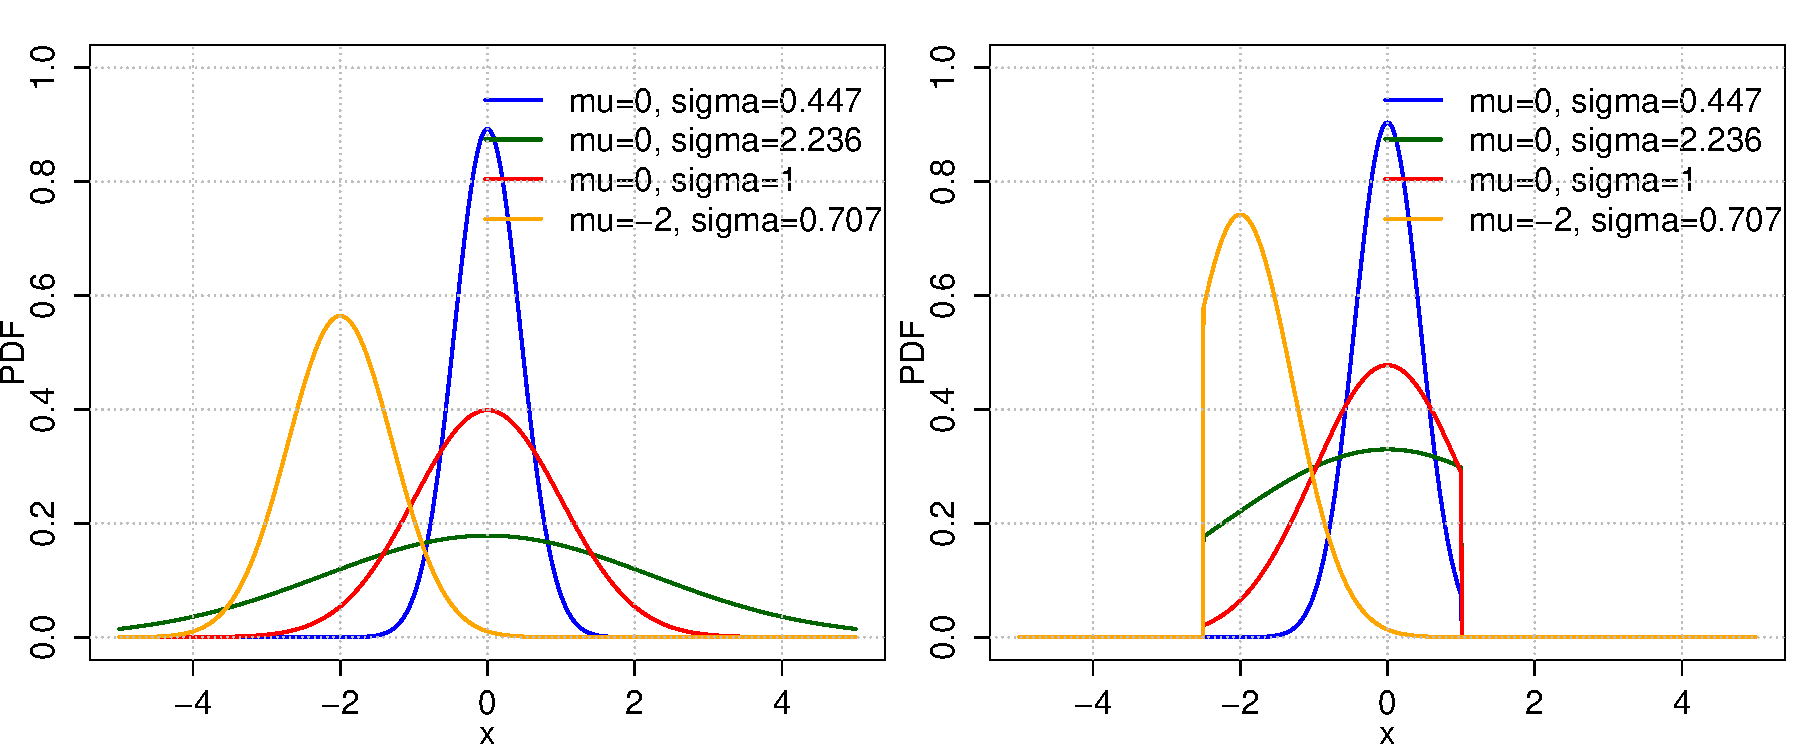
\includegraphics[width=140mm]{pics/TruncatedNormal1.pdf}
\caption{Truncated normal distribution, N1. The truncated density plots on the right hand side
were performed using the \emph{truncnorm} function of the \emph{dtruncnorm} R-package.}
\vspace{-1em}
\label{fig:truncatedNormal1}
\end{figure}


%%%%%%%%%%%%%%%%%%%%%%%%%%%%%%%%%%%%%%%%%%%%%%%%%%%%%%%%%%%%%%%%%%%%%%
\section{Independency of ProbOnto}
\label{sec:ProbOntoIndependent}
It is worth to stress that ProbOnto ontology and knowledge base are fully 
independent from PharmML. The provided schema is  tailored towards
the needs of PharmML and is otherwise entirely optional. 
ProbOnto doesn't enforce a certain way to implement it from
a tool designer -- this allows it to be used across the DDMoRe target tools, languages
and beyond. 

